% AAMAS 2013 Manuscript

% This file should be compiled with "aamas2013.cls" 
% ----------------------------------------------------------------------
% REMEMBER: After having produced the .bbl file,
% and prior to final submission, you *NEED* to 'insert'
% your .bbl file into your source .tex file so as to provide
% ONE 'self-contained' source file.
% ----------------------------------------------------------------------

%%%%%%%%%%%%%%%%%%%%%%%%%%%%%%%%%%%%%%%%%%%%%%%%%%%%%%%%%%%%%%%%%%%%%%%%%%%%%%
% STYLE NOTES
%
% TENSE AND VOICE
% * Actual experimental events
% 	We wrote descriptions of actual experimental events using past tense, in 
%	active voice, as the first person plural.
%
% * All other contexts
%	We write all other text using present tense, in active voices, as the
%	the first person plural.  
%
% CONVENTIONS
% flapping-wing, small-scale, lightweight, MAV
%
%%%%%%%%%%%%%%%%%%%%%%%%%%%%%%%%%%%%%%%%%%%%%%%%%%%%%%%%%%%%%%%%%%%%%%%%%%%%%%
% SETUP
\documentclass{aamas2013}

%----------------------------------------------------------------------------%
% PACKAGES
\usepackage{color}
\usepackage[pdftex]{hyperref}
\usepackage{amsmath}
\usepackage{amssymb}
\providecommand{\norm}[1]{\lVert#1\rVert}

%----------------------------------------------------------------------------%
% METADATA
\def \papertitle{Cooperative Control for Narrow Passage Traversal with an 
Ornithopter Micro Air Vehicle and Lightweight Ground Station}
\def \paperkeywords{AAMAS proceedings, multiagent systems, cooperative control, 
particle filter, micro air vehicle, ground station, visual servoing, pose 
estimation, flapping wing, ornithopter, biomimetic}
\def \paperterms{Algorithms, Performance, Design, Experimentation}
\def \paperauthors{Ryan C. Julian, Cameron J. Rose, Humphrey Hu, and Ronald S. Fearing}

% Set title
\title{\papertitle}

% PDF bookmarks
\definecolor{linkCol}{gray}{0.25}
\hypersetup{
    pdftitle={\papertitle},
    pdfauthor={\paperauthors},
    pdfsubject={\paperterms},
    pdfkeywords={\paperkeywords},
    pdfpagemode=UseOutlines, bookmarksopen, bookmarksnumbered,
    colorlinks, linkcolor=linkCol, citecolor=linkCol, urlcolor=linkCol
}

%----------------------------------------------------------------------------%
% pdfLatex clean-up 
\pdfpagewidth=8.5truein
\pdfpageheight=11truein

\begin{document}

%%%%%%%%%%%%%%%%%%%%%%%%%%%%%%%%%%%%%%%%%%%%%%%%%%%%%%%%%%%%%%%%%%%%%%%%%%%%%%
% AUTHORS

%% Paper number instead of authors
%\numberofauthors{1}
%\alignauthor Paper  580

\numberofauthors{4}
\author{
\alignauthor Ryan C. Julian\\
       \affaddr{Department of EECS}\\
       \affaddr{Univ. of California, Berkeley}\\
       \affaddr{Berkeley, CA 94720}\\
       \email{ryanjulian@berkeley.edu}
\alignauthor Cameron J. Rose\\
       \affaddr{Department of EECS}\\
       \affaddr{Univ. of California, Berkeley}\\
       \affaddr{Berkeley, CA 94720}\\
       \email{c\_rose@eecs.berkeley.edu}
\alignauthor Humphrey Hu\\
       \affaddr{Robotics Institute}\\
       \affaddr{Carnegie Mellon University}\\
       \affaddr{Pittsburgh, PA 15213}\\
       \email{humhu@cmu.edu}
\and
\alignauthor Ronald S. Fearing\\
       \affaddr{Department of EECS}\\
       \affaddr{Univ. of California, Berkeley}\\
       \affaddr{Berkeley, CA 94720}\\
       \email{ronf@eecs.berkeley.edu}
}

%%%%%%%%%%%%%%%%%%%%%%%%%%%%%%%%%%%%%%%%%%%%%%%%%%%%%%%%%%%%%%%%%%%%%%%%%%%%%%
% TITLE
\maketitle

%%%%%%%%%%%%%%%%%%%%%%%%%%%%%%%%%%%%%%%%%%%%%%%%%%%%%%%%%%%%%%%%%%%%%%%%%%%%%%
% ABSTRACT
\begin{abstract}
The power, size, and weight constraints of micro air vehicles (MAVs) limit 
their on-board sensing and computational resources. Ground vehicles have 
less mobility than MAVs, but relaxed size constraints and typically more 
computing power, creating opportunities for cooperation. In this work, we 
demonstrate cooperative target-seeking between a 13 gram ornithopter MAV 
and a lightweight ground station using computer vision.

We also introduce a new ornithopter MAV, the 13 gram H$^2$Bird. It 
features clap and fling wings, improves upon a previous design by 
utilizing a carbon fiber airframe, tail rotor, and elevator, and carries a 
payload of 2.8 grams. We augment the ornithopter's built-in 
gyroscope-based control with a ground station, which has power and weight 
requirements appropriate for deployment on a millirobotic ground vehicle. The ground 
station provides heading estimates to the ornithoper by running a 
real-time motion tracking algorithm on a live video stream. This allows 
the ornithopter to reliably negotiate flight through narrow openings.

We demonstrate the performance of the location estimation and navigation 
algorithms. We model the backwards-reachable region for successfully 
navigating through narrow openings. Finally, we verify this model through 
with experiments with narrow passage traversal.
\end{abstract}
%%%%%%%%%%%%%%%%%%%%%%%%%%%%%%%%%%%%%%%%%%%%%%%%%%%%%%%%%%%%%%%%%%%%%%%%%%%%%%
% ACM METADATA

% Note that the category section should be completed after reference to 
% the ACM Computing Classification Scheme available at
% http://www.acm.org/about/class/1998/.
% A category including the fourth, optional field follows...
%\category{D.2.8}{Software Engineering}{Metrics}[complexity measures, 
% performance measures]
\category{I.2.9}{Robotics}{Autonomous Vehicles}
\category{I.2.9}{Robotics}{Distributed Artificial Intelligence}[Multiagent Systems]
\category{I.2.9}{Robotics}{Vision and Scene Understanding}[Motion]

% General terms should be selected from the following 16 terms: 
% Algorithms, Management, Measurement, Documentation, Performance, 
% Design, Economics, Reliability, Experimentation, Security, 
% Human Factors, Standardization, Languages, Theory, Legal Aspects, 
% Verification.
\terms{\paperterms}

% Keywords are your own choice of terms you would like the paper to be indexed 
% by.
\keywords{\paperkeywords}

%%%%%%%%%%%%%%%%%%%%%%%%%%%%%%%%%%%%%%%%%%%%%%%%%%%%%%%%%%%%%%%%%%%%%%%%%%%%%%
\section{Introduction}
\begin{figure}[!tb]
\centering
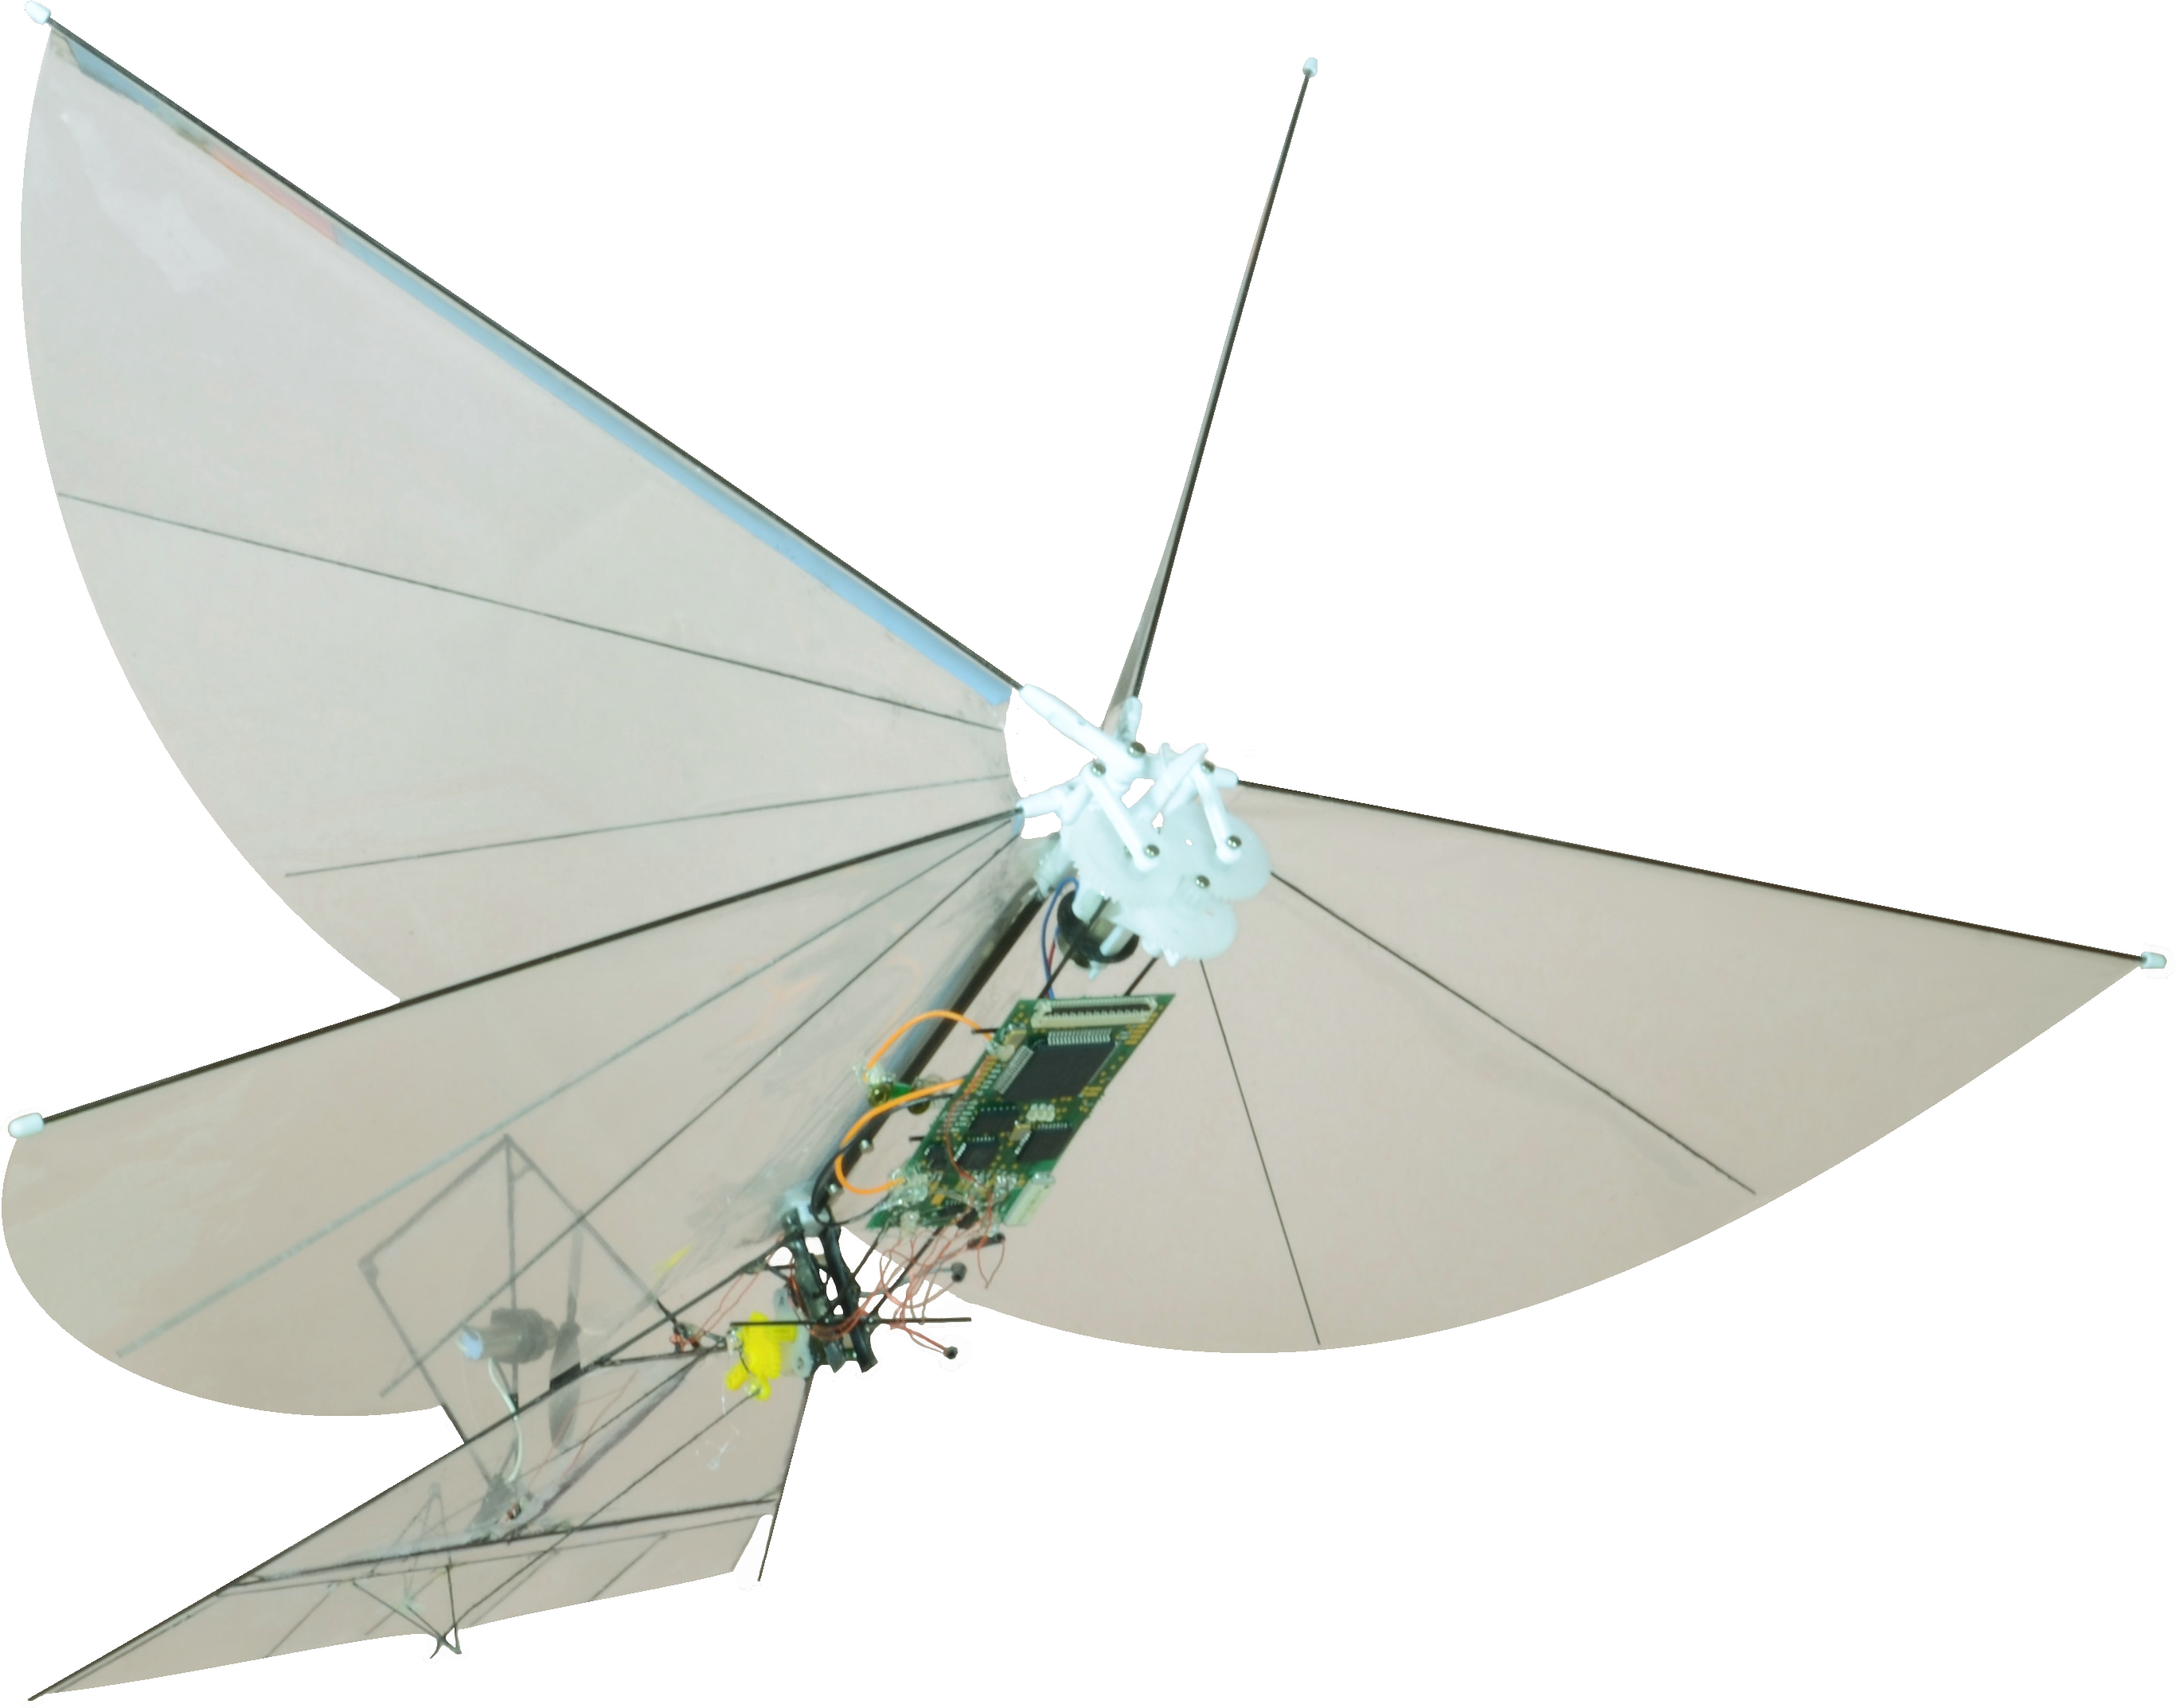
\includegraphics[width=\linewidth]{figures/h2bird.png}
\caption{H$^2$Bird ornithopter MAV}
\label{fig:h2bird}
\end{figure}
Power, size, and weight constraints for micro air vehicle (MAV) 
platforms are amongst the most restrictive of all robotic platforms. With
significantly limited sensing and computing capabilities, only the most rudimentary
control and state estimation algorithms can be executed on-board these platforms. 
Even more restrictive are the constraints for flapping wing MAVs, 
a class of MAVs that exhibit demonstrate safety and noise profiles superior to those
of rotor craft MAVs, but at the expense of reduced payload weight.

Compounding these engineering restrictions are the many non-linear
flight dynamics exhibited by flapping wing flight~\cite{humbert:dipteran2}\cite{cheng:tandrdamping}. 
Much past research on flapping wing MAVs has been focused on overcoming the 
difficulties associated with controlling and modeling in the face of these 
non-linearities\cite{floreano:flying}. Common approaches to simplify these 
dynamic models include averaging over the wingbeat period~\cite{Schenato:flightcontrol}
\cite{cheng:tandrdamping}, and using linear, low-dimensional models to predict the 
behavior in flight~\cite{Shigeoka:ornithopter}. Advances have lead to the
development of some high-performance platforms, such as the sub-15 gram DelFly 
as described by deCroon et al.~\cite{delfly:design}. 

Many of the control laws that previous researches have developed from the
dynamic models of flapping-winged flight, such as periodic forcing and other
control methods as described %TODO you need to use real names, it's not kosher to refer to citation numbers directly
in~\cite{doman:dynamics}\cite{khan:longitudinal_control}\cite{leonard:averaging}, are computationally complex and
require powerful on-board computing. In our work, we develop a simpler, less
computationally intensive method of control for negotiating narrow passages.

In contrast, there is considerably less previous work on guidance of flapping wing MAVs. 
Baek demonstrated altitude control with an external camera~\cite{baek:altitude}. 
de Croon et al. demonstrated obstacle avoidance with an onboard camera and offboard 
processing~\cite{delfly:avoid}. For sub-20 gram ornithopters, Baek et al. 
\cite{baek:tracking} is one of the few examples of scompletely autonomous target seeking.

There also exists a body of work on guidance and control for fixed wing and rotary wing 
MAV platforms, but many of these methods make extensive use of GPS or motion capture systems
~\cite{kingston:timeattitude}\cite{kanade:3dvision}. While operating indoors, using
GPS to estimate the pose of the MAV is not possible, and motion capture
requires expensive and stationary modification of the environment. The power
and payload limits on flapping wing MAVs make on-board sensing difficult, so multi-agent
cooperative control schemes are apt solutions.

\cite{Jung1998Range}\cite{Hyams1999Cooperative}\cite{Mehta2006Adaptive}
\cite{Rudol2008Micro}\cite{Luo2011Air}

%TODO Add in final paragraph to lead-in to our work

%%%%%%%%%%%%%%%%%%%%%%%%%%%%%%%%%%%%%%%%%%%%%%%%%%%%%%%%%%%%%%%%%%%%%%%%%%%%%%
\section{Robotic and Vision Platforms}
%----------------------------------------------------------------------------%
\subsection{H$^2$Bird Ornithoper}
% humphrey
In order to conduct these experiments on cooperation, we designed a new
flapping-wing MAV, known as the H$^2$Bird. Built around the Silverlit i-Bird 
RC flyer power train and clap-fling 
wings\footnote{\raggedright Silverlit Toys Manufactory Ltd.: i-Bird RC Flyer
\href{http://www.silverlit-flyingclub.com/wingsmaster/}
     {http://www.silverlit-flyingclub.com/wingsmaster/}}, 
the H$^2$Bird's wingspan is 26.5 cm and it has a flight weight of 13 grams. A 
tail propeller and servo-controlled tail elevator provide control in the yaw 
and pitch axes. The on-board ImageProc 2.4\footnote{ImageProc 2.4: \\
\href{https://github.com/biomimetics/imageproc\_pcb}
     {https://github.com/biomimetics/imageproc\_pcb}} 
electronics package consists of a 40 MIPS microprocessor, 6 DOF IMU, 
IEEE 802.15.4 radio, VGA camera, and motor drivers, all powered by a 90 mAh 
lithium polymer battery. In routine flight, the H$^2$Bird averages 1.2 m/s 
ground speed, and can operate for approximately 10 minutes.
%TODO footnote for ImageProc

%----------------------------------------------------------------------------%
\subsection{Ground Station Computer Vision Platform}
% ryan
Cooperative behavior is a promising strategy for autonomous navigation of 
unexplored and unstructured environments. We intend that this system will be 
fully mobile in these environments, not tied to a static ground station or 
motion capture laboratory. To demonstrate the feasibility of this approach, 
we designed our ground station to conform to the power and weight 
constraints of highly mobile millirobotic ground vehicles, such as 
OctoRoACH, which can traverse rough terrains with speed and agility~\cite{Pullin2012Dynamic}. 

Rather than power-intensive PC processors, we used the ARM-based 
BeagleBoard single-board computer as reference computation platform. The
BeagleBoard consumes approximately 1 watt while running our computer vision 
and control algorithms. It uses the same processor as popular sub-10 gram 
processor modules---such as the Gumstix Overo and LogicPD Torpedo---which are 
light enough for deployment on millirobotic ground vehicles. We pair the 
BeagleBoard with an off-the-shelf consumer USB web camera, for similar image 
quality and resolution to the miniature camera modules available at 
millirobot scale. The BeagleBoard communicates with the H$^2$Bird using a 
USB radio module which implements the IEEE 802.15.4 wireless standard.
%TODO footnotes: Gumstix, LogidPD

Our ground station software is based on the Ubuntu Linux\footnote{\raggedright Ubuntu: 
Canonical Ltd., \href{http://www.ubuntu.com/}{http://www.ubuntu.com/}} distribution
modified with a custom version of the Linux kernel. We use the Python
\footnote{\raggedright Python: Python Software Federation, \href{http://www.python.org/}
{http://www.python.org/}} programming language for control, robot communication, 
and telemetry, and the OpenCV\footnote{\raggedright OpenCV: Willow Garage, 
\href{http://opencv.willowgarage.com/wiki/}{http://opencv.willowgarage.com/wiki/}} 
computer vision libraries for image capture and processing.
%%%%%%%%%%%%%%%%%%%%%%%%%%%%%%%%%%%%%%%%%%%%%%%%%%%%%%%%%%%%%%%%%%%%%%%%%%%%%%
\section{System Concept and Algorithms}
%TODO ryan

\begin{figure}[tb]
\centering
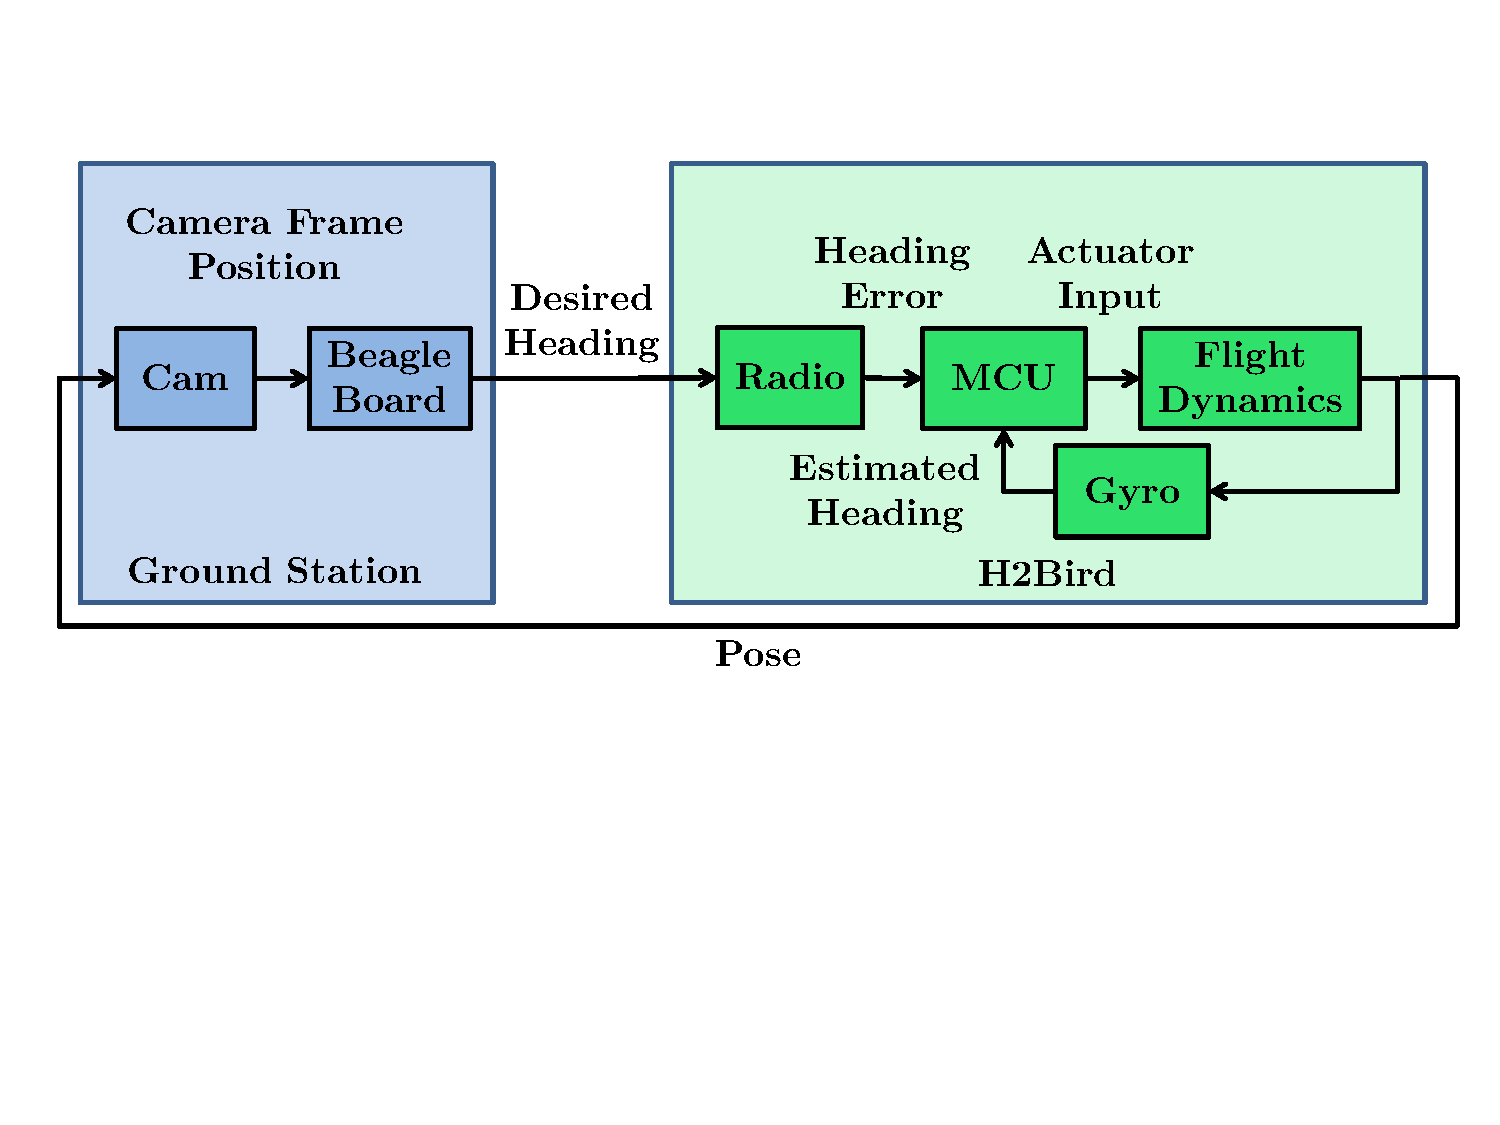
\includegraphics[width=\linewidth]{figures/process_flow.pdf}
\caption{Overview of the cooperative control system.}
\label{fig:process_flow}
\end{figure}
%TODO h2bird label in diagram should have superscript

%----------------------------------------------------------------------------%
\subsection{Ornithoper Attitude Control}

\begin{figure}[!tb]
\centering
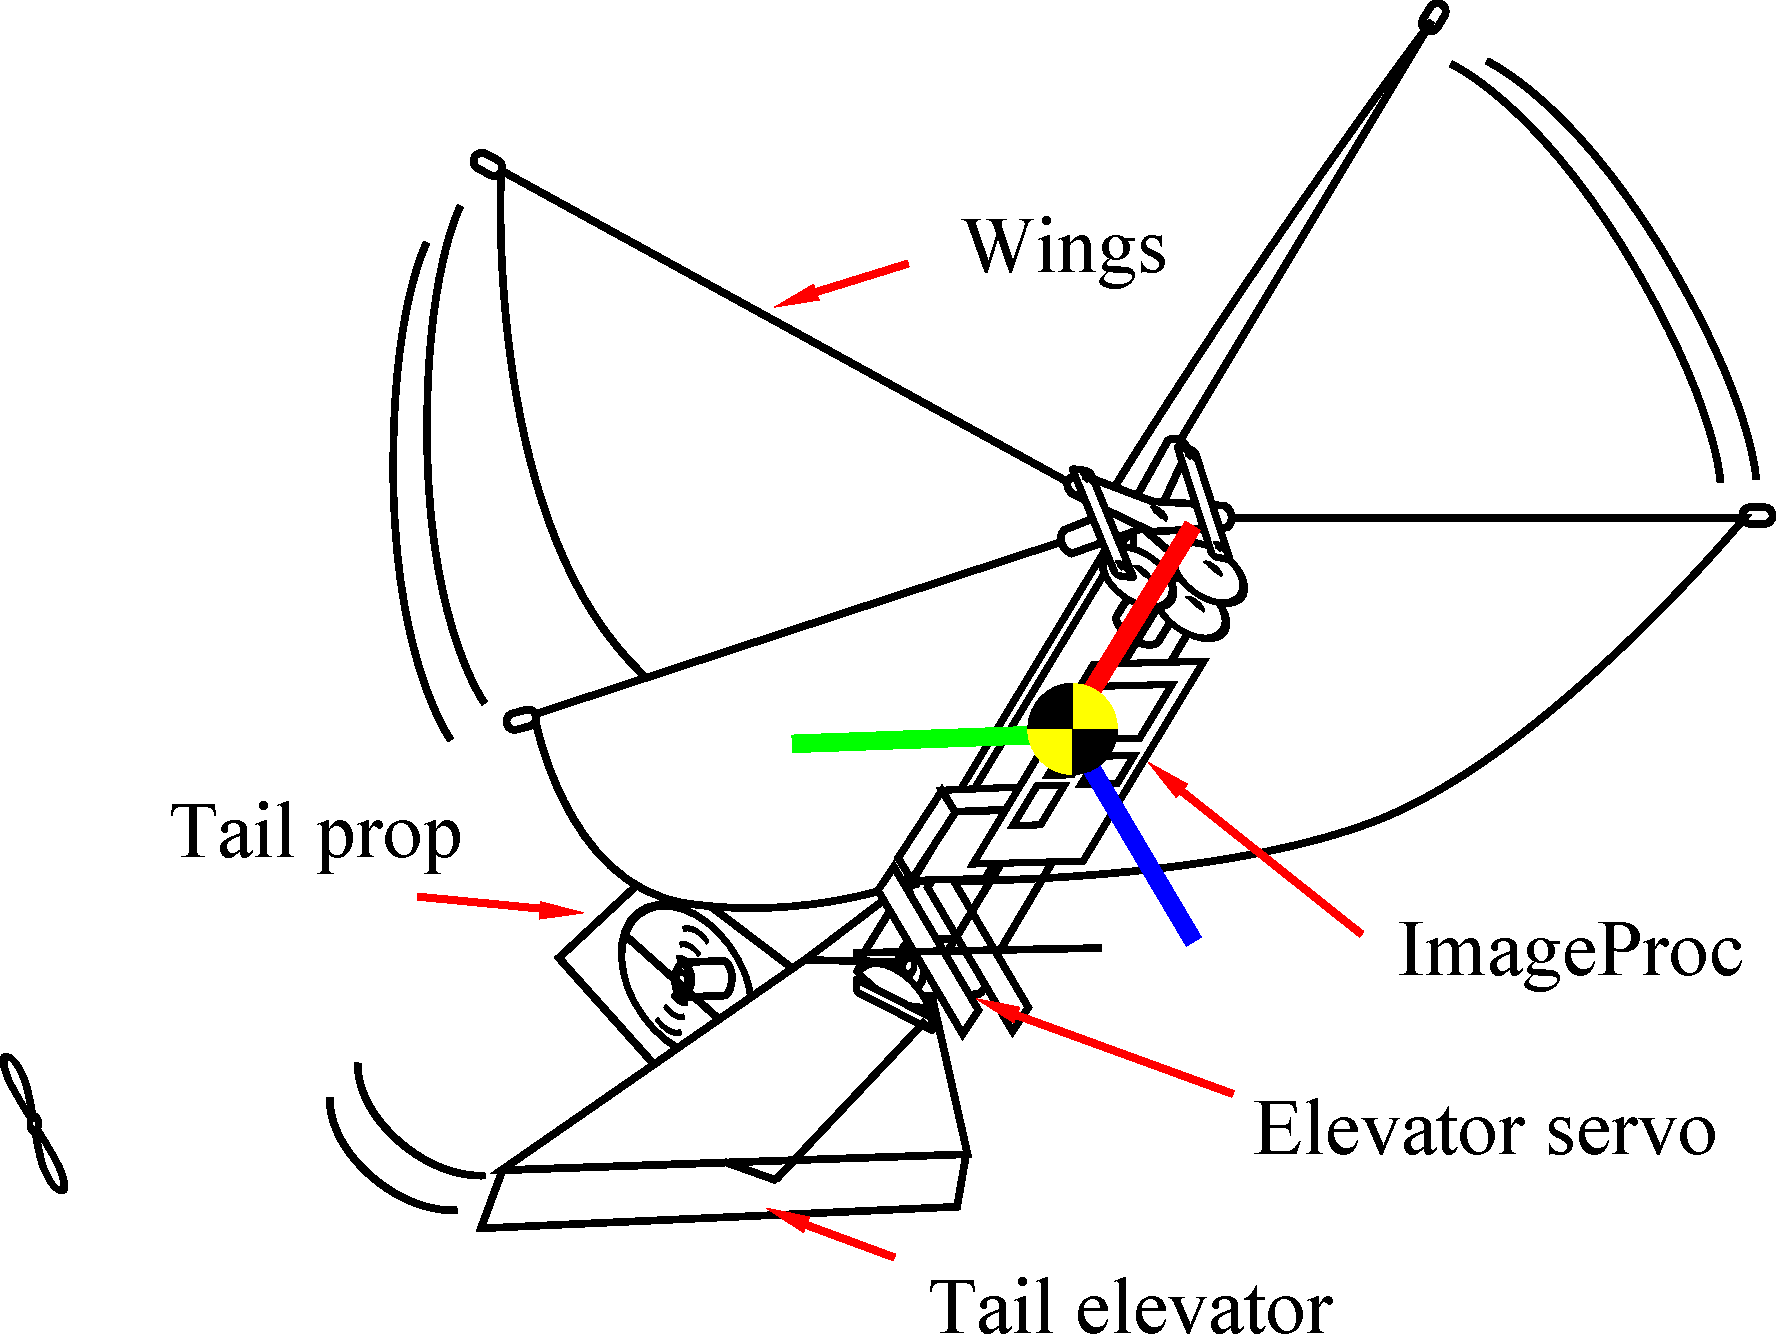
\includegraphics[height=150pt]{figures/h2bird_axes.pdf}
\caption{H$^2$Bird ornithopter with attitude control axes and labeled control surfaces.}
\label{fig:h2Bird_axes}
\end{figure}
%TODO label h2bird drawing

Attitude estimation and control for the H$^2$Bird runs on-board to achieve 
maintain high sample rate attitude control. We estimate the vehicle pose by naively
integrating the IMU, and use a proportional plus integral plus derivative (PID) 
controller for controlling the vehicle.

The high pitch angles flapping wing flyers achieve in routine flight distinguish them 
from other MAVs. Baek demonstrated control on a similar vehicle using PID and an Euler angle
parameterization of orientation~\cite{baek:tracking}. However, Euler angle parameterizations of the vehicle orientation 
suffer from singularities around these high pitch angles, so we instead 
represent the vehicle orientation with quaternions. An additional benefit of 
the quaternion representation is its ability to represent relative body and 
world coordinate angular displacements compactly with quaternion multiplication.

Our implementation of quaternion-based control is similar to Knoebe's~\cite{knoebe:quatcontrol}:
Given a reference pose represented in quaternion form $q_r$, we define the error as the rotation $q_e$ 
required to reach the reference pose from the estimated pose $q$ (Eq.~\ref{eq:quat_error}). 
\begin{align}
\label{eq:quat_error}
q_e &= q^{\prime}\cdot q_r \\
		&= q_{e,w} + q_{e,x}\hat{i} + q_{e,y}\hat{j} + q_{e,z}\hat{k} \notag 
\end{align}
We then convert this error quaternion to an angle axis representation and use this 
as input to the PID controller (Eqs.~\ref{eq:quat_linearize} and~\ref{eq:quat_angle}).
These calculations are performed onboard with trigonometric lookup tables for speed.
\begin{align}
\label{eq:quat_linearize}
Q_e &= \alpha\cdot q_e/\sin(\alpha /2) \\
		&= \alpha_{x}\hat{i} + \alpha_{y}\hat{j} + \alpha_{z}\hat{k} \notag
\end{align}
\begin{equation}
\label{eq:quat_angle}
\alpha = 2\arccos(q_{e,w})
\end{equation}

%----------------------------------------------------------------------------%
\subsection{Ground Station Pose Estimation}
The ground station performs simple two-dimensional pose estimation on 
H$^2$Bird using a particle filter-based motion tracking algorithm. This pose 
estimate is the feedback input to the cooperative visual servoing feedback 
loop (Sec. \ref{sec:visual_servoing_concept}). We limit our pose estimation 
approach to monocular two-dimensional object tracking in pixel space. This 
allows us to perform real-time video tracking using the modest computational 
resources available on the ground station, and similarly millirobotic ground 
vehicles.

Our pose estimation algorithm tracks H$^2$Bird motion in the frame using a 
particle filter~\cite{thrun2005probabilistic}. We initialze particles 
uniformly across the frame. To improve numerical stability, we normalize the 
weights of all particles on each iteration, and only resample the particle 
population when the mean particle weight falls below a pre-determined 
threshold.

%............................................................................%
\subsubsection{Motion Model}
Our motion model (Eq.~\ref{eq:motion_model}) is a simple Gaussian transition 
centered around each particle's current position, augmented with an 
$\epsilon$-random uniform sampling strategy. In Eq.~\ref{eq:motion_model}, 
$x^{[i]}_t$ is the state of the $i^\text{th}$ particle at time $t$, $\Sigma$ 
is a chosen covariance matrix, and $b$ is vector of the height and width of 
the camera frame.
\begin{equation}
\label{eq:motion_model}
x^{[i]}_t \sim \begin{cases}
\mathcal{N}(x^{[i]}_{t-1}, \Sigma), &\text{with probability } 1-\epsilon \\
\mathcal{U}(0,b),& \text{with probability } \epsilon \\
\end{cases}\\
\end{equation}
The experiments presented in this work use a diagonal covariance matrix 
with a variance of 256, and an $\epsilon$ of 0.3. We find that the Gaussian 
transition model is sufficient for tracking motion in which frame-to-frame 
position changes are relatively small. The $\epsilon$-random uniform 
transitions increase tracking robustness, by forcing the filter to always 
sample all of the pixel space. This prevents overconfidence and collapse, 
and decreases reacquisition delay. 

%............................................................................%
\subsubsection{Emission Model}
Our emission model (Eq.~\ref{eq:emission_model}) implements a sampling
approach to motion tracking via na\"{i}ve background subtraction[CITATION].
\begin{equation}
\label{eq:emission_model}
w^{[i]}_t = 1 + \norm{f_0(x^{[i]}_t)-f_t(x^{[i]}_t)}^2
\end{equation} 
The system provides the emission model with $f_0$, the frame representing 
the background and $f_t$, the most recent frame captured. The model assigns 
a weight $w^{[i]}_t$ to each particle $x^{[i]}_t$, proportional to the color 
distance in RGB space between the pixels of $f_0$ and $f_t$ at the location 
$x^{[i]}_t$. Hence, particles are more likely to be resampled in portions of 
the image which appear different from the background.

For the experiments presented in this work, we assumed that neither the bird 
nor any other moving object were visible in the first frame captured on system 
start. We saved the first frame captured by the system, and provided it as 
the background frame $f_0$ for every iteration of the particle filter. This 
resulted in a sampling approach to na\"{i}ve background subtraction. 

Na\"{i}ve background subtraction is brittle to changes in the scene over 
time[CITATION]. However, we found it very efficient, and reliable enough for the 
short time spans necessary for H$^2$Bird to successfully negotiate narrow 
openings, which are typically less than five seconds. Substituting $f_0$ 
with a more sophisticated extraction of the background would implement a 
more sophisticated approach to background subtraction, with no changes to 
the underlying motion tracking filter.

%----------------------------------------------------------------------------%
\subsection{Cooperative Visual Servoing}
\label{sec:visual_servoing_concept}
Remote guidance of the H$^2$Bird is performed by commanding relative changes in the
reference orientation. With estimates of the vehicle pose, we calculate an altitude
error and horizontal error. The ground station then commands incremental changes to 
the H$^2$Bird pitch and yaw are according to a PID control law, with positive altitude error
corresponding to negative pitch increments and positive horizontal error
corresponding to negative yaw increments. We window the controller integrator term 
to prevent windup when the bird is being launched, and tuned the derivative term
to dampen oscillations associated with the system latency [?].

\begin{figure}[tb]
\centering
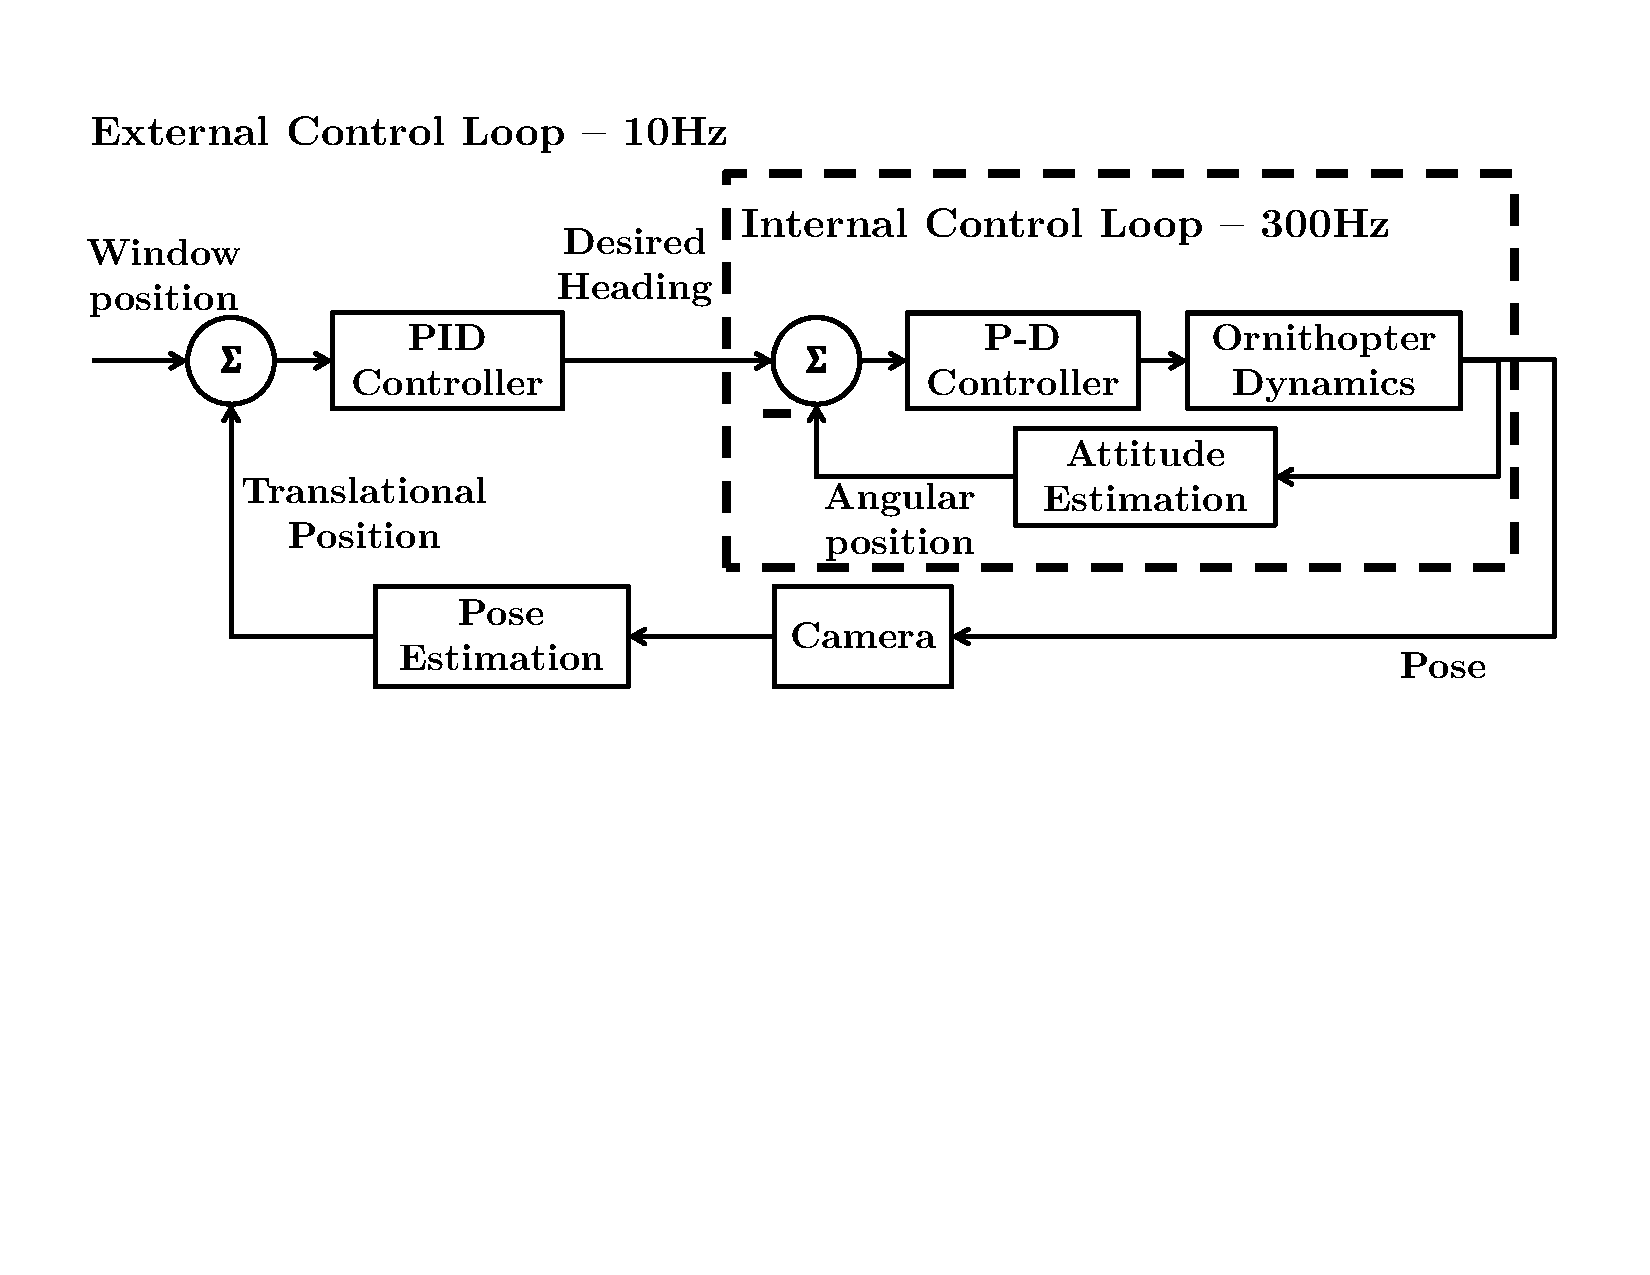
\includegraphics[width=\linewidth]{figures/block_diagrams.pdf}
\caption{Overall block diagram of the cooperative control system.}
\label{fig:block_diagram}
\end{figure}

\begin{figure}[tb]
\centering
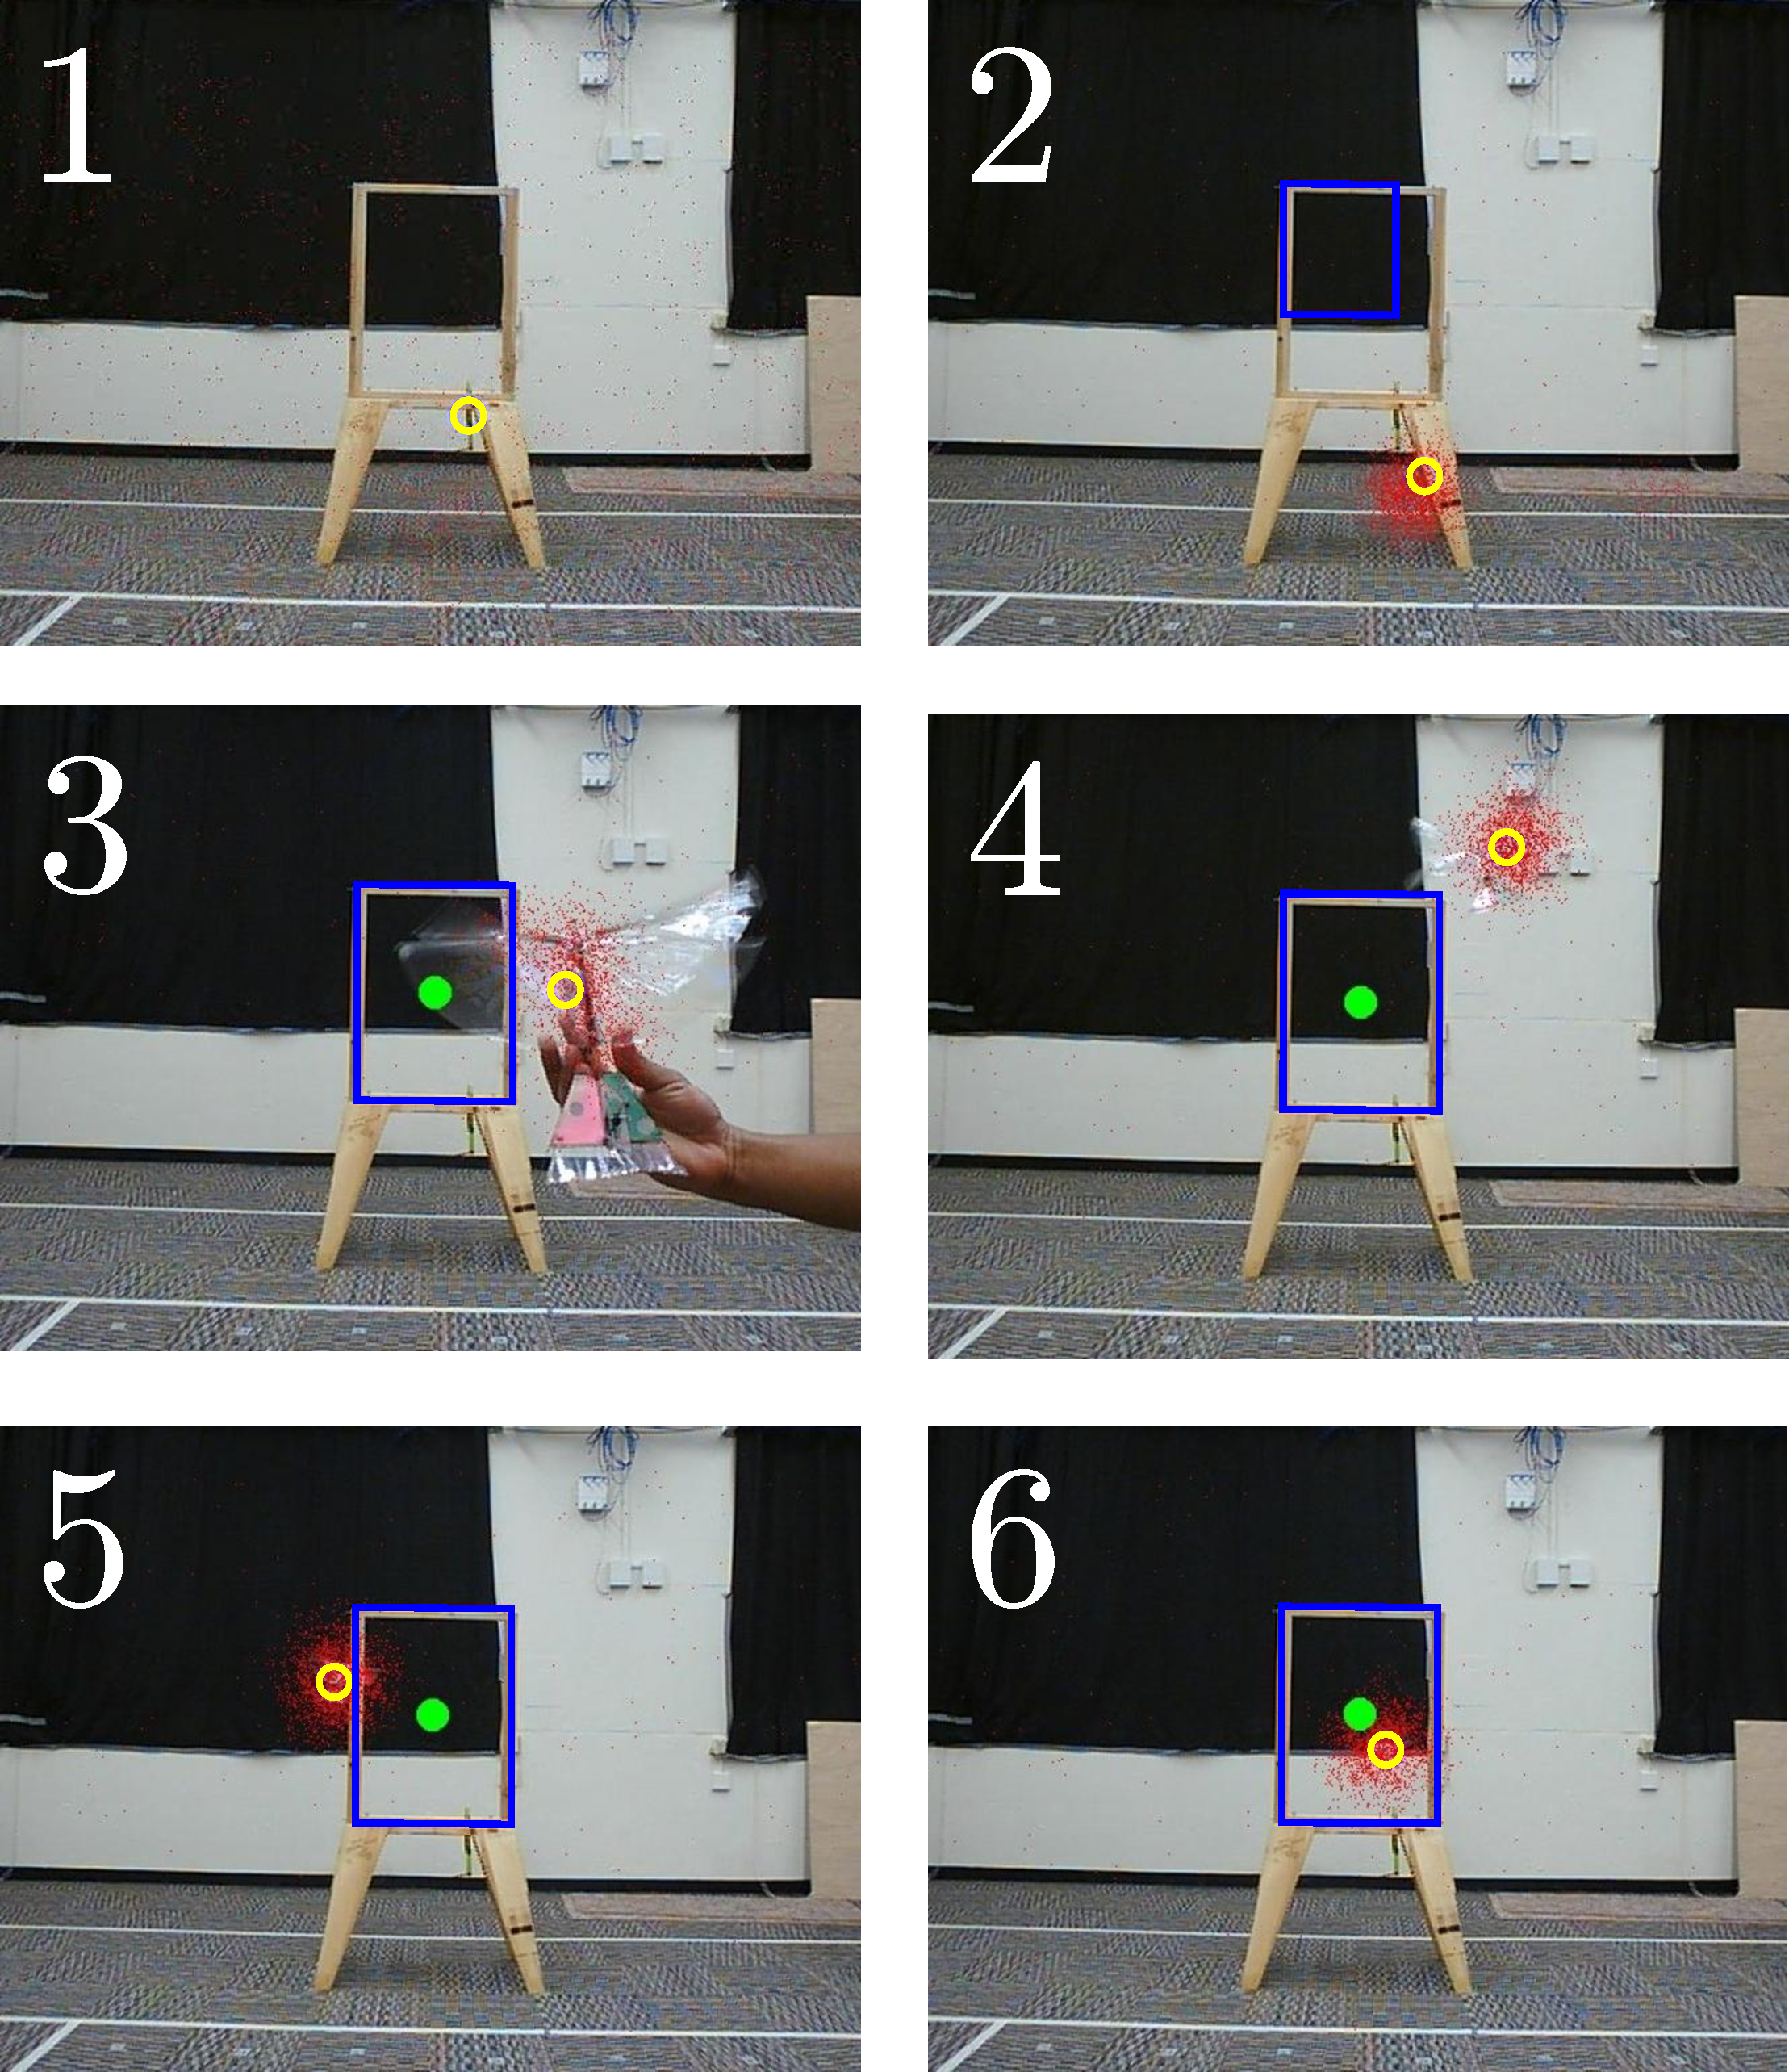
\includegraphics[width=\linewidth]{figures/pf_screencap.pdf}
\caption{Frame sequence from video feed used for tracking. Particles 
are shown in \textcolor{red}{red}, the current state estimate as a 
\textcolor{yellow}{yellow} circle, the window bounding box in
\textcolor{blue}{blue}, and the target location as a \textcolor{green}{green} 
circle. 1.~Particles initialized uniformly across the frame; 2.~Human operator 
dragging bounding box across the window; 3.~H$^2$Bird enters the frame. 
Particles converge on its location; 4.~Release H$^2$Bird, which 
begins cooperative autonomous flight toward the target; 5.~Visual servoing 
controller overshoots the window on the left, and commands a right-turn 
maneuver to recover; 6.~H$^2$Bird successfully navigates through the window.}
\label{fig:pf_screencap}
\end{figure}

%%%%%%%%%%%%%%%%%%%%%%%%%%%%%%%%%%%%%%%%%%%%%%%%%%%%%%%%%%%%%%%%%%%%%%%%%%%%%%
\section{System Model}
\label{sec:system_model}

%----------------------------------------------------------------------------%
\subsection{Ornithopter Attitude Control}
\label{sec:model_attitude}

To model the yaw motion of the ornithopter, we developed a one-dimensional model using the physical heading angle as the output and the heading angle set by the ground station as the input. This model accounts for both the yaw dynamics of the ornithopter and the internal PID controller on the actuator inputs for the tail rotor. We decided upon a one-dimensional model to reduce the complexity of the overall model and enable simple angle inputs and outputs, which is similar to our methods during experimentation. The model format is shown in Equation~\ref{eq:plain_model}.

\begin{equation}
\label{eq:plain_model}
H(s) = \frac{K}{1 + Rs}
\end{equation}

To model the translational position of the ornithopter, we used a form of Dubin's car model~\cite{lavalle:planning} with the angular position, $\theta$ as an input rather than a state. The overall motion of the system can be modeled as shown in Equation~\ref{eq:total_model_plain}, where $\theta$ is the time domain output of (\ref{eq:plain_model}) with the angular setpoint provided by the ground station as the input.

\begin{equation}
\label{eq:total_model_plain}
\begin{aligned}
& \dot{x} = sin(\theta)\\
& \dot{y} = cos(\theta)\\
\end{aligned}
\end{equation}

%----------------------------------------------------------------------------%
\subsection{Ground Station Pose Estimation}

The model of the ground station combines both the camera model and the
computational model for pose estimation. The camera model contains both a
latency, which would occur in between the "camera" and "ornithopter dynamics"
in Fig.~\ref{fig:block_diagram}, and a model for the viewing angle. We model the 
viewing angle for the camera as a pixel map from one edge of a
63$^{\circ}$ viewing triangle to the other. The camera has an image width of
640 pixels. The desired heading angle in degrees for a given distance from the
camera is calculated according to Equation~\ref{eq:desired_heading}, where $d$
is the distance of the robot in front of the camera and $x$ is the horizontal
position of the robot relative to the center of the window in meters. This
relation reflects the fact that the camera cannot determine the depth of the
robot.

\begin{equation} \label{eq:desired_heading} \text{Desired heading} =
\frac{640\text{px}}{2*\text{d}*\tan{\frac{63^{\circ}}{2}}}*\frac{63^{\circ}}{640\text{px}}*\text{x}
\end{equation}

The computational model accounts for the latency added by the operations required to
run the particle filter and calculate the input to send to the robot. 

%----------------------------------------------------------------------------%
\subsection{Cooperative Visual Servoing}



%%%%%%%%%%%%%%%%%%%%%%%%%%%%%%%%%%%%%%%%%%%%%%%%%%%%%%%%%%%%%%%%%%%%%%%%%%%%%%
\section{Experiments}

%----------------------------------------------------------------------------%
\subsection{System Identification}

%............................................................................%
\subsubsection{Ornithoper Attitude Control}

We determined the turning speed and turning radius of the H$^2$Bird
experimentally using the response of the system to the step input of a
clockwise 90 degree turn. To measure the response of the system, we recorded
the angular position data of the ornithopter calculated from the on-board
gyroscope data. We then used
MATLAB\footnote{The MathWorks, Inc. Matlab:
\href{http://www.mathworks.com/products/matlab/}
     {http://www.mathworks.com/products/matlab/}} to fit a
simple low-order model to the step response as discussed in Sec.~\ref{sec:model_attitude}.

%............................................................................%
\subsubsection{Ground Station Pose Estimation}

To measure the capture latency of the camera, we alternatively flashed black
and white color in front of the camera and measured the time lapse before it
detected the color change. We averaged this result over 50 trials to determine
the capture latency.

To compute the particle filter latency, we used system timers to determine the
average time from the start of computation to the end of computation.

%............................................................................%
\subsubsection{Cooperative Visual Servoing}

%----------------------------------------------------------------------------%
\subsection{Model Verification}

We tested our cooperative visual servoing system with a simple target seeking
experiment: the H$^2$Bird must fly through a specified obstacle, in this case,
a wooden frame meant to simulate a window. As the H$^2$Bird cannot detect the
target on its own, we used the ground station to provide remote headings for
navigation to the window. Ground truth data was collected via a motion capture
system in the test room. A sketch of the experimental setup is shown in
Fig.~\ref{fig:experiment_cartoon}.

% TODO clarify or roll into paragraph
Each trial included the following steps:
\begin{enumerate}
\item The window is identified by the user. 
\item The H$^2$Bird is released in view of the camera by hand at the desired starting grid point.
\item The H$^2$Bird attempts to fly to the window with remote guidance from
the base station.
\end{enumerate}

In total, we ran 80 trials over a variety of starting positions. The goal of
our experiments was to verify the model described in
Secttion~\ref{sec:system_model}, so we conducted 60 of the 80 trials in a grid
along the edges of the camera viewplane in 0.05 meter increments from the
window to determine the success rate on the edges of the testing space. We
conducted 20 additional trials directly in front of the camera to determine
the success rate near the center of the testing space. After every 5 trials,
we replaced the current battery with a fully charged one.

\begin{figure}[tb]
\centering
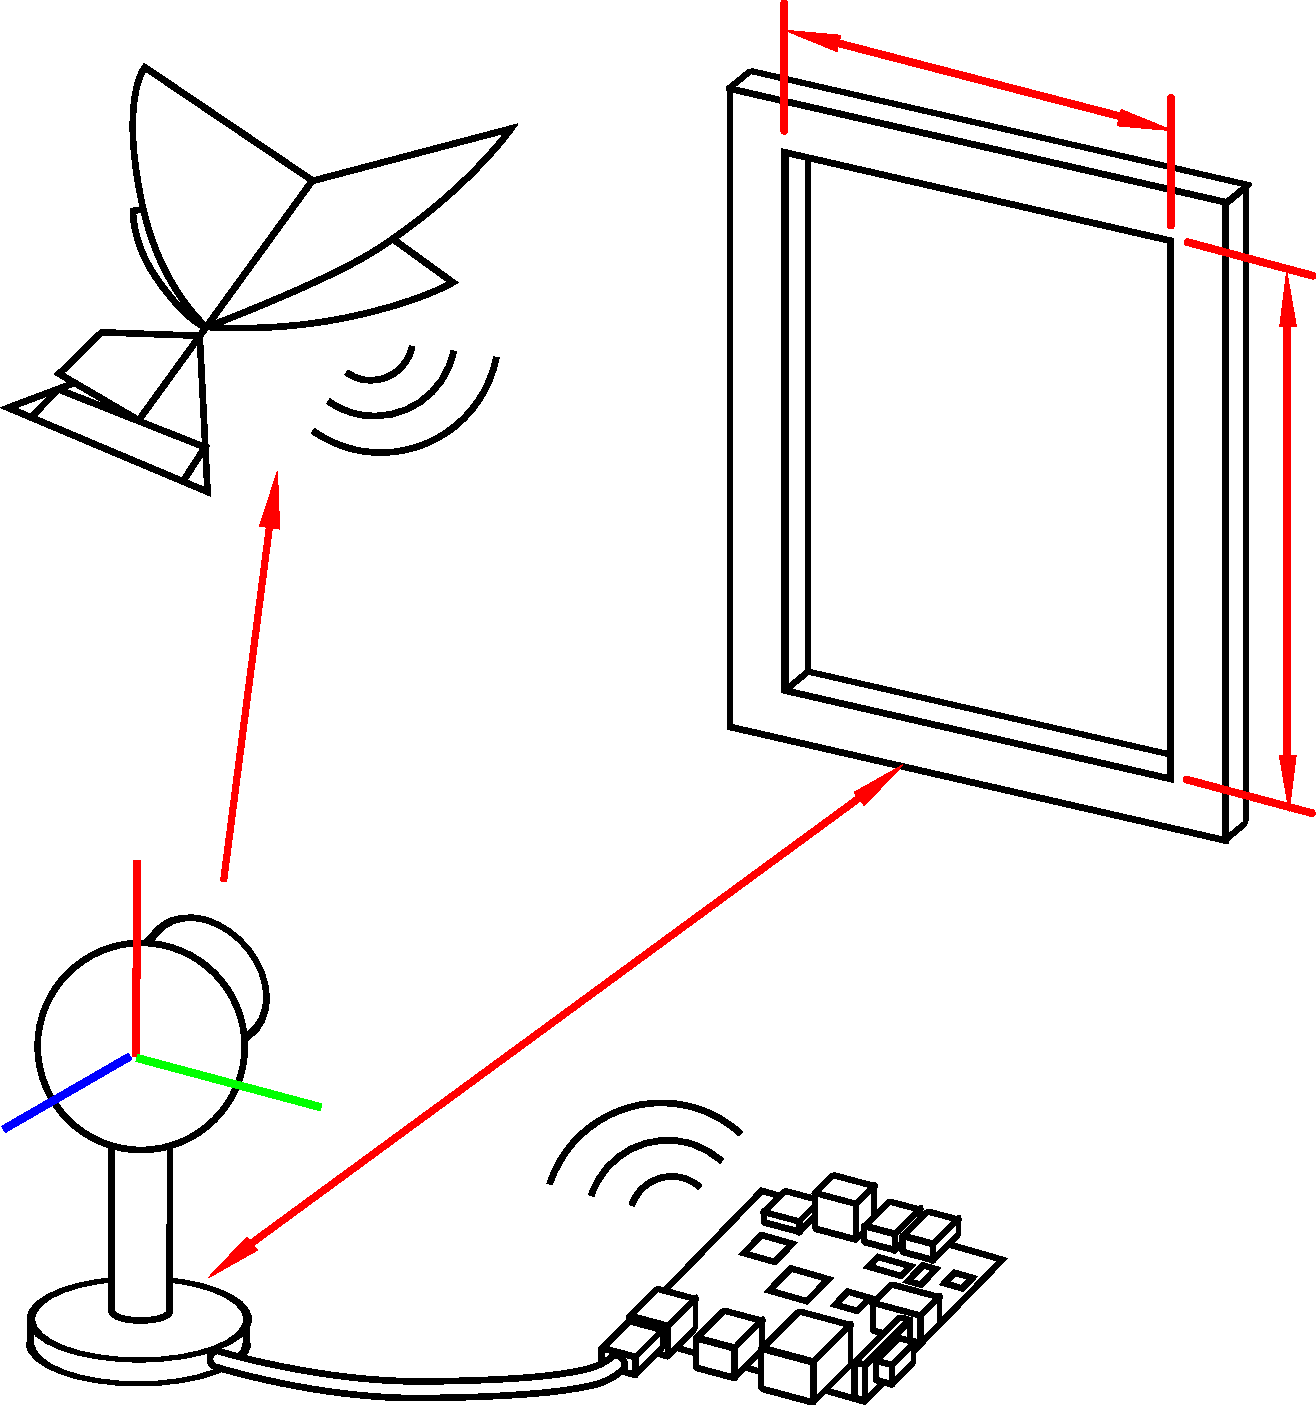
\includegraphics[width=\linewidth]{figures/experiment_cartoon.pdf}
\caption{Conceptual sketch of experimental setup.}
\label{fig:experiment_cartoon}
\end{figure}
%TODO label experiment cartoon

%%%%%%%%%%%%%%%%%%%%%%%%%%%%%%%%%%%%%%%%%%%%%%%%%%%%%%%%%%%%%%%%%%%%%%%%%%%%%%

%%%%%%%%%%%%%%%%%%%%%%%%%%%%%%%%%%%%%%%%%%%%%%%%%%%%%%%%%%%%%%%%%%%%%%%%%%%%%%
\section{Results and Performance}
\label{sec:performance}
%TODO cameron
To bound the performance of the cooperative control system, we determine 
the feasible set of initial conditions that result in successful narrow 
passage traversal using both analytical and empirical methods. We conducted 
experiments to validate this model.

The following sections detail how we calculated the feasible and infeasible
regions using system identification and present the results of our
experimental trials.

%----------------------------------------------------------------------------%
\subsection{System Identification}

%............................................................................%
\subsubsection{Ornithoper Attitude Control}
\label{sec:flight_control}
%TODO cameron
\begin{figure}[tb]
\centering
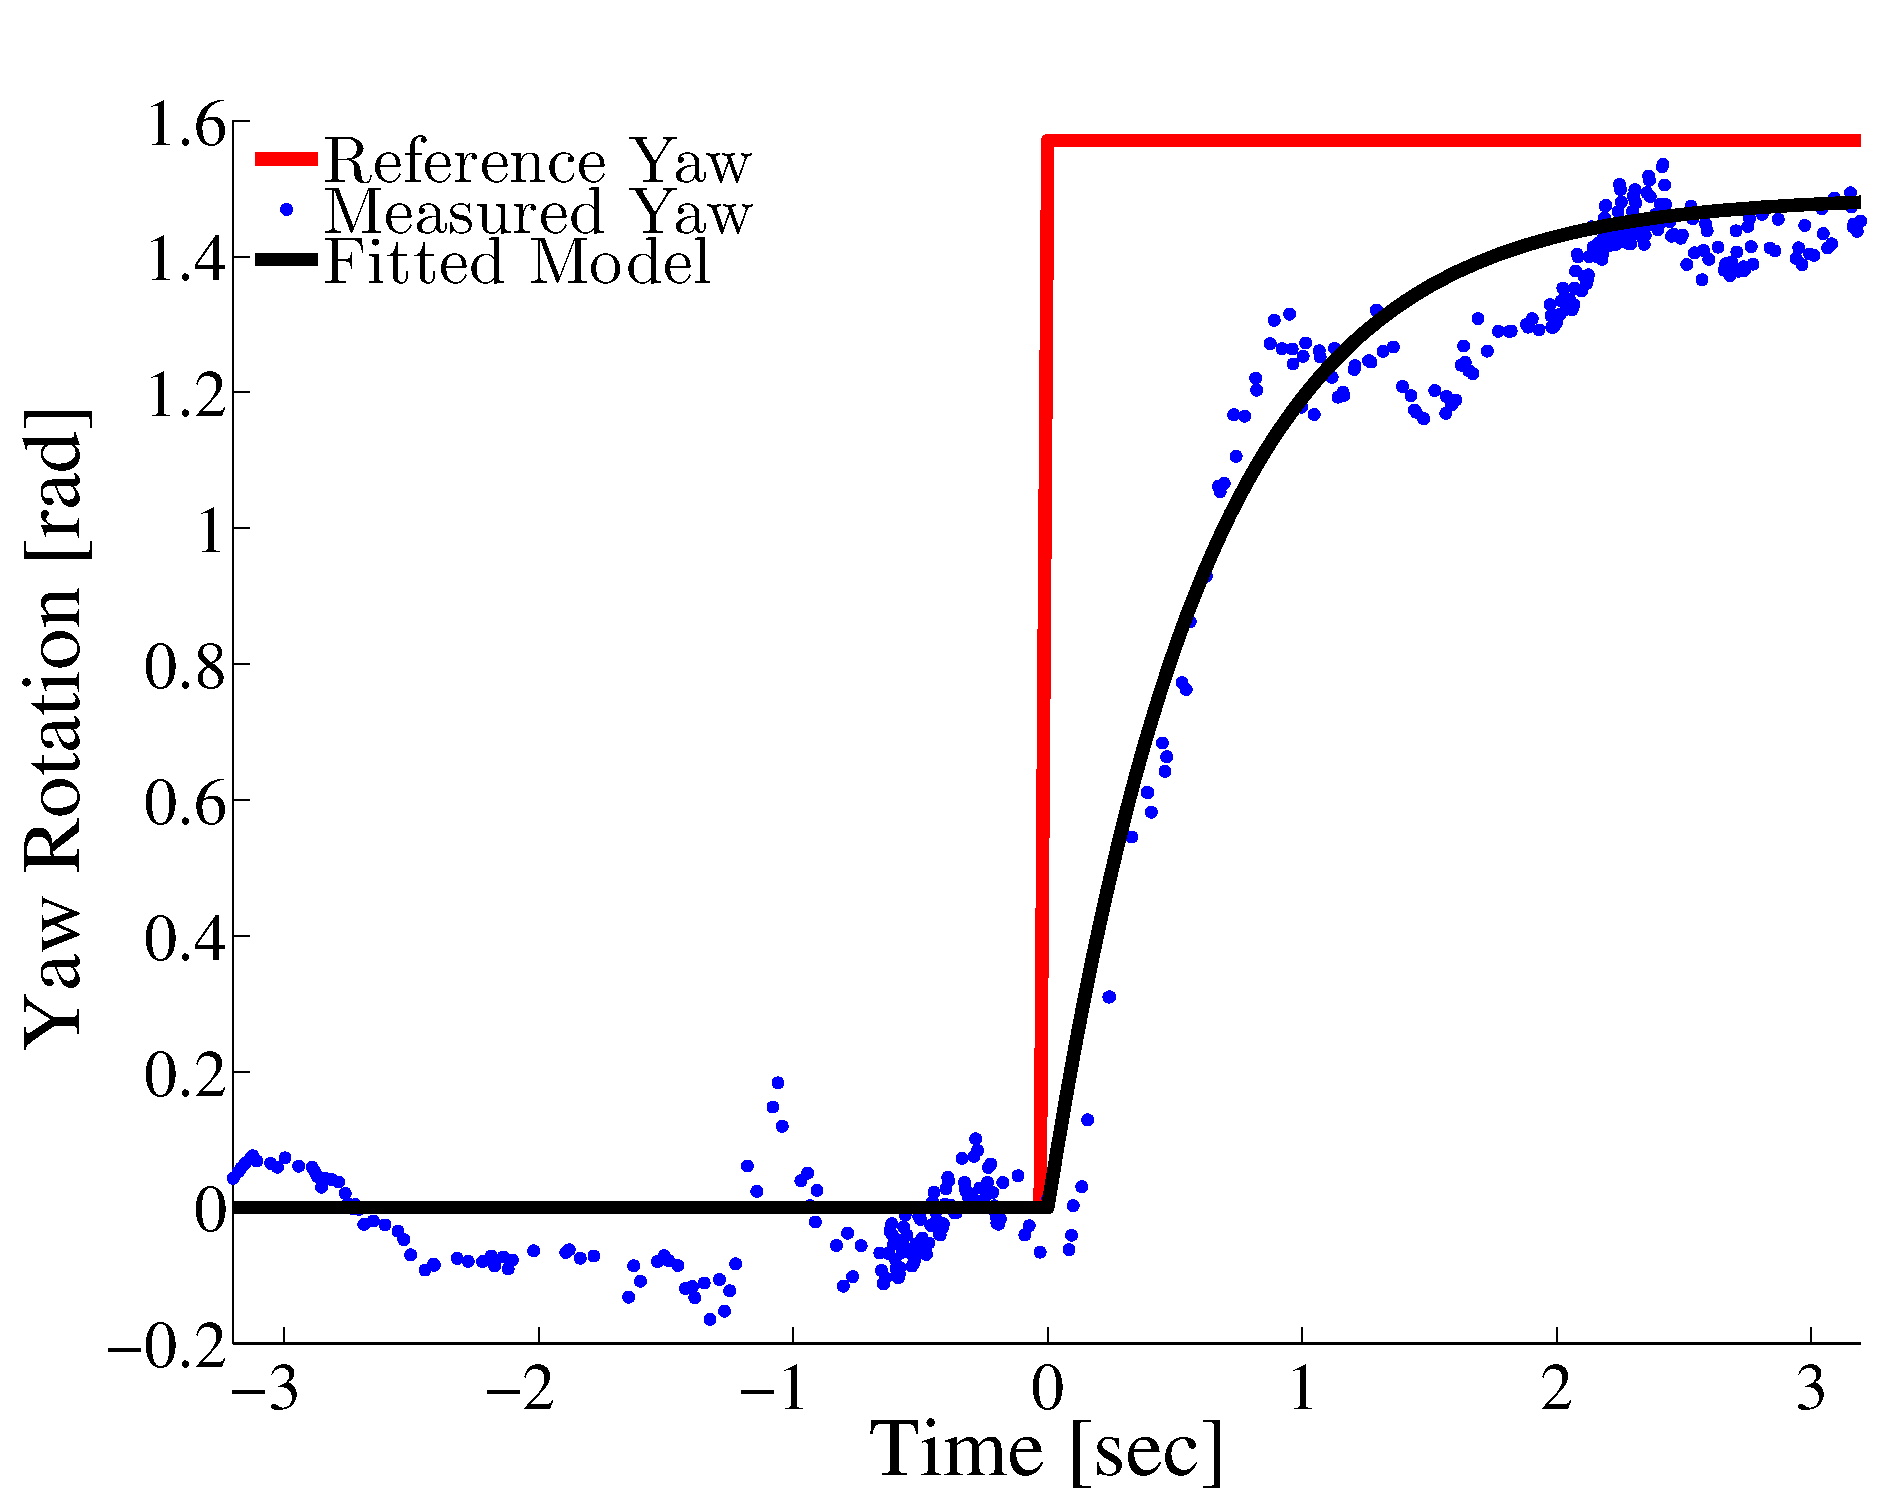
\includegraphics[width=\linewidth]{figures/step_response_total.pdf}
\caption{H$^2$Bird step response}
\label{fig:step_response}
\end{figure}
%TODO reduce number of sig figs

The results of the step response experiment are described in
Fig.~\ref{fig:step_response}. The first-order model that we fit to the
response is in Equation~\ref{eq:transfer_func}.

\begin{equation}
\label{eq:transfer_func}
H(s) = \frac{0.95}{1+0.62s}
\end{equation}

The step response rise time is 1.4 seconds. The H$^2$Bird flies
at an average forward velocity of 1.2 m/s during our experiments, so the
estimated minimum turning radius of the robot is 1.07 maters, as described in
Equation~\ref{eq:min_radius}. In the experiments, we choose a flight speed
lower than the maximum speed of the ornithopter, to facilitate more robust
tracking.

\begin{equation}
\label{eq:min_radius}
\begin{aligned}
\text{Minimum radius} & = \frac{360^{\circ}*\text{Rise time}*\text{Flight
speed}}{\text{Final angle}*2*\pi}\\
& = \frac{360^{\circ}*1.4s*1.2\frac{m}{s}}{90^{\circ}*2*\pi} = 1.07 m
\end{aligned}
\end{equation}

%............................................................................%
\subsubsection{Ground Station Pose Estimation}

The latency that we measured for the camera was 25ms, and the measured
partiicle filter computational latency was 12.5ms.

%............................................................................%
\subsubsection{Cooperative Visual Servoing}
\label{sec:visual_servoing}

\begin{figure*}[tb]
\begin{minipage}[b]{0.45\linewidth}
\centering
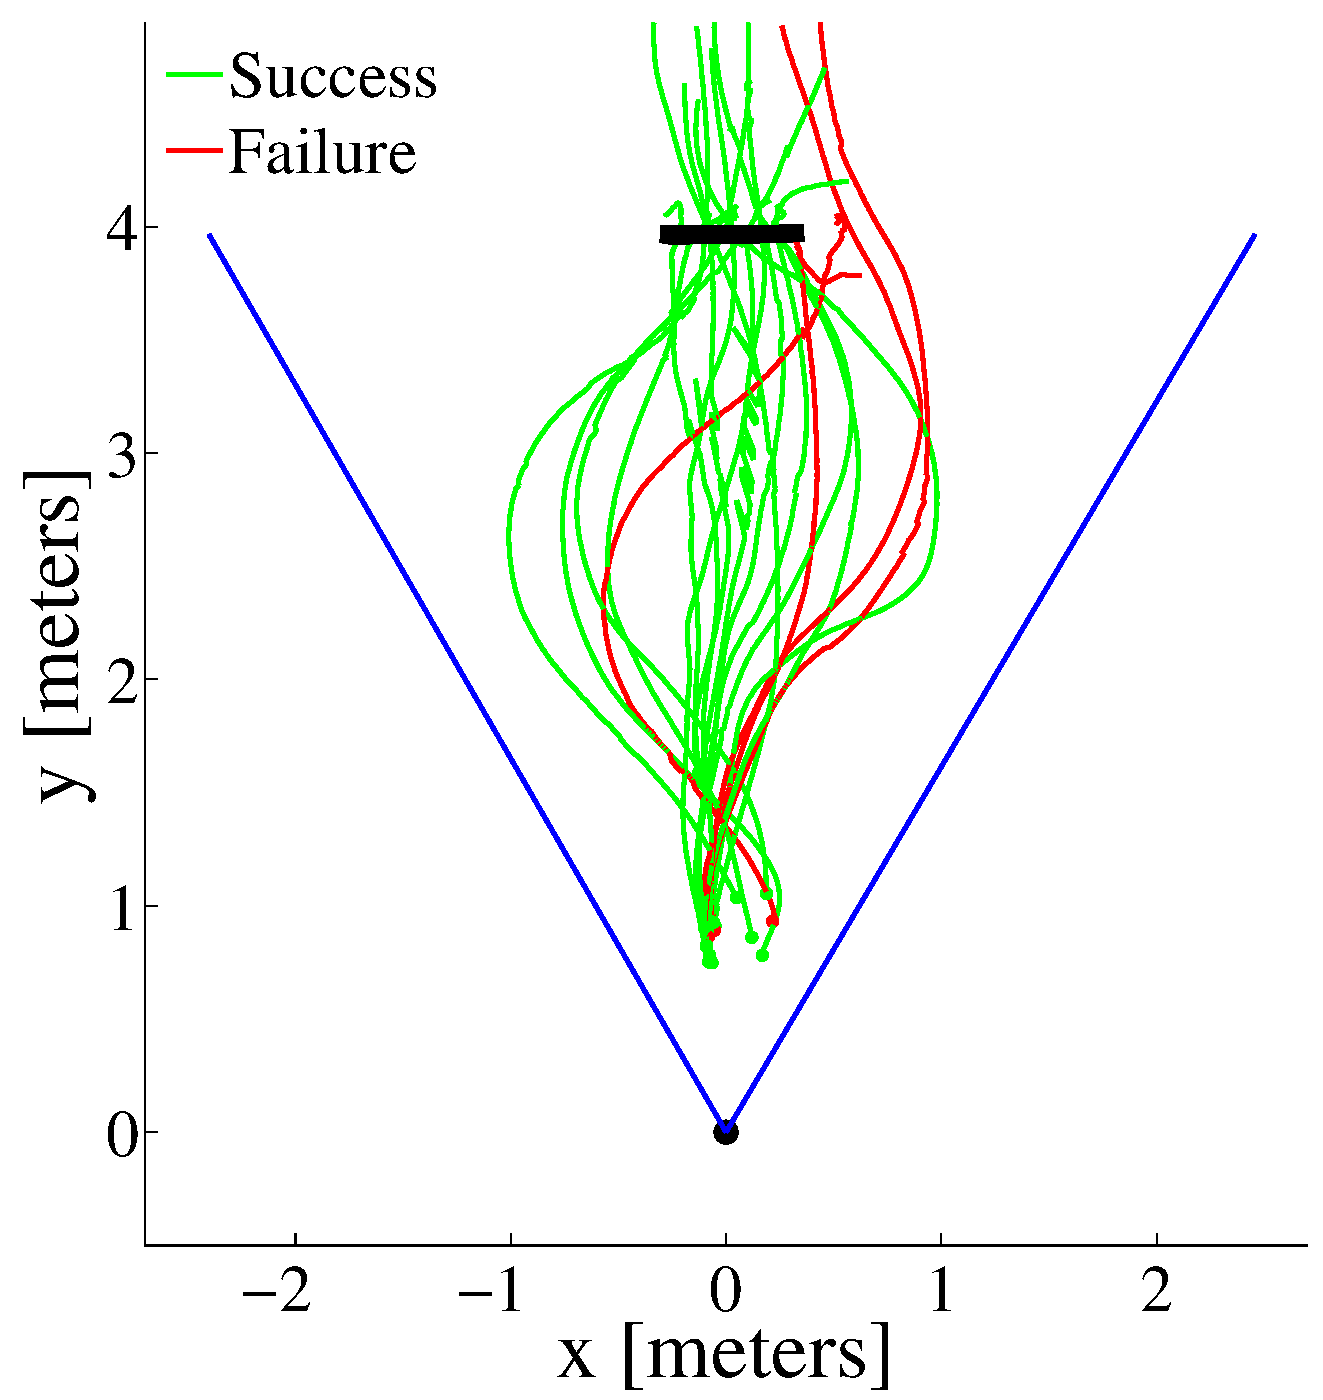
\includegraphics[width=\linewidth]{figures/flight_paths_feasible.pdf}
\caption{Plot of camera field of view and experimental trials within the feasible region.}
\label{fig:flight_paths_feasible}
\end{minipage}
\hfill
\begin{minipage}[b]{0.45\linewidth}
\centering
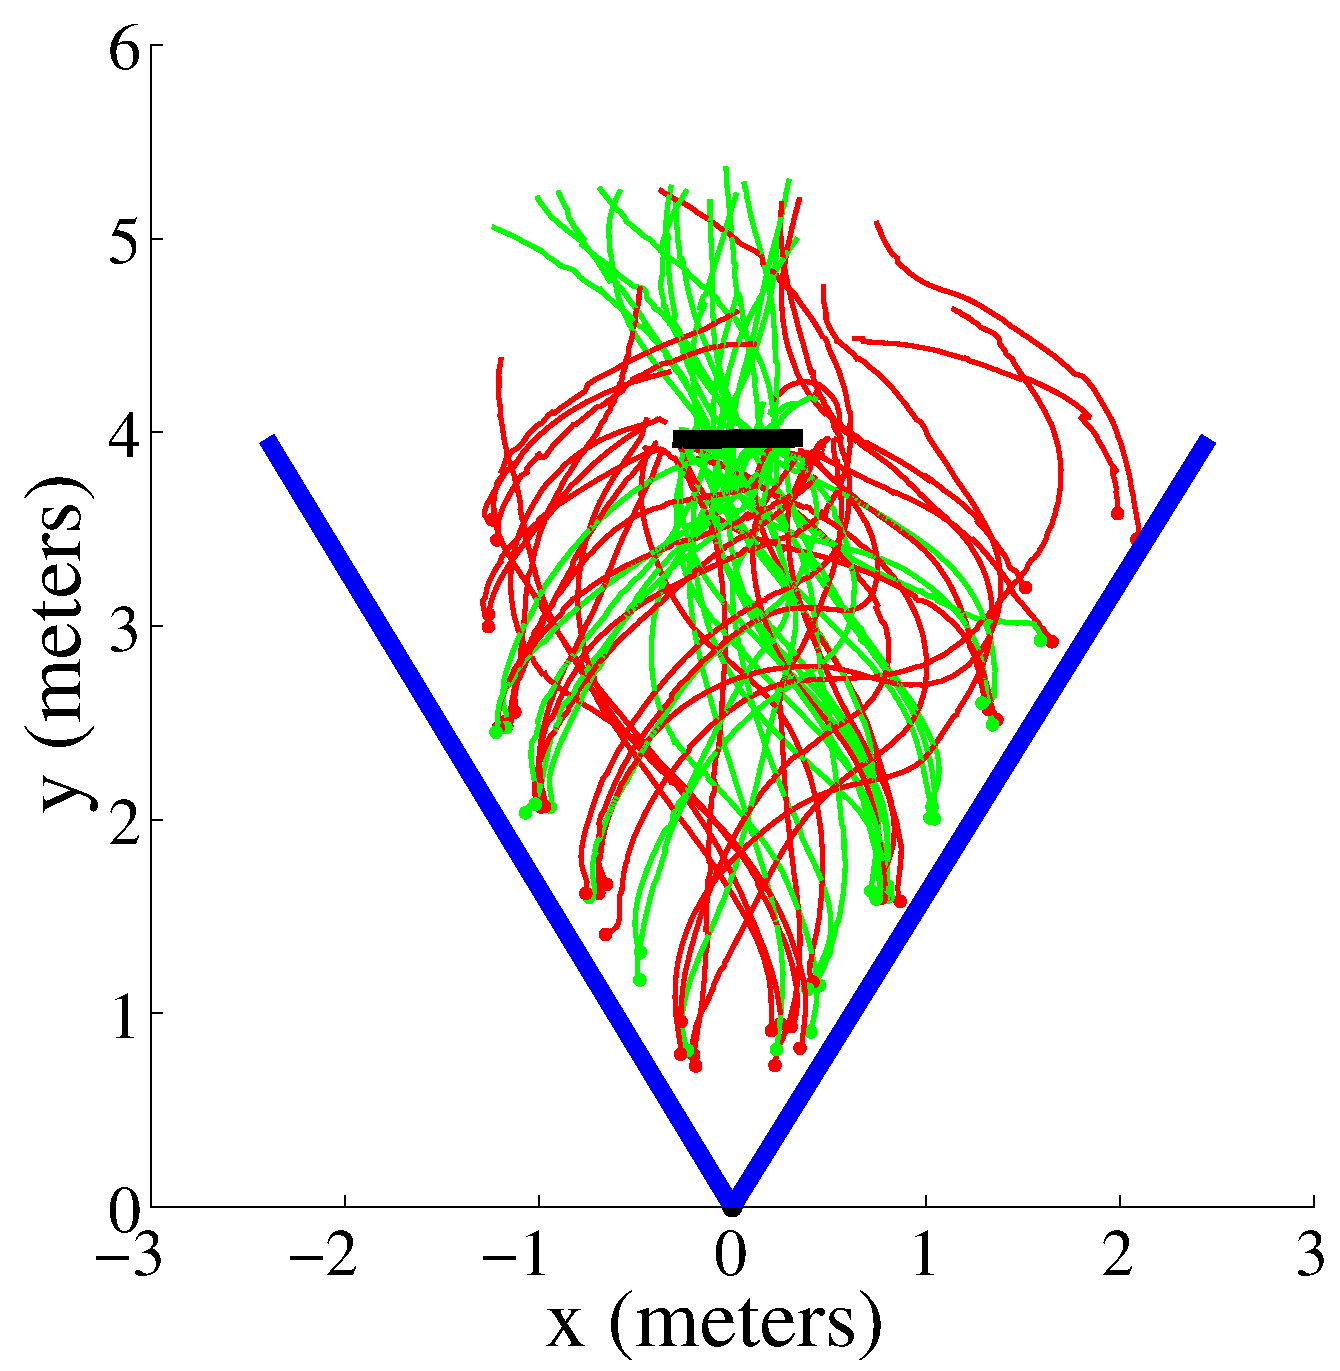
\includegraphics[width=\textwidth]{figures/flight_paths.pdf}
\caption{Plot of camera field-of-view and perimeter experimental trials overlayed.}
\label{fig:flight_paths}
\end{minipage}
\end{figure*}

The results of our experimental trials are shown in
Figs.~\ref{fig:flight_paths} and~\ref{fig:flight_paths_feasible}. For
initial conditions in the middle of the testing space and in front of the
camera, we achieved a success rate of 80\%. This case is depicted in
Fig.~\ref{fig:flight_paths_feasible}. As we moved towards the edges of the
feasible region in Fig.~\ref{fig:flight_paths}, the success rate diminishes
to 50\% because of several factors. On the edges of the camera frame, the yaw
control inputs are large in magnitude, although this is not necessary in all
cases. Since the control algorithm we are using has no notion of depth, it
applies the same control input whether the ornithopter is close to the camera,
where small changes in heading are adequate, or far away from the camera,
where large changes in heading are necessary. Due to this phenomenon, the
controller often over or under-compensates in certain regions, depending upon
the PID tuning and the distance from the camera. Tracking noise can also cause
passage negotiation to fail. Variations in the H$^2$Bird hand launch can cause
the system to respond differently for similar initial conditions. In addition,
the H$^2$Bird battery was changed approximately every 5 tests, adding more
variation to the H$^2$Bird performance by affecting the motor power output.

%----------------------------------------------------------------------------%
\subsection{Model Verification}

\begin{figure*}[tb]
\begin{minipage}[b]{0.45\linewidth}
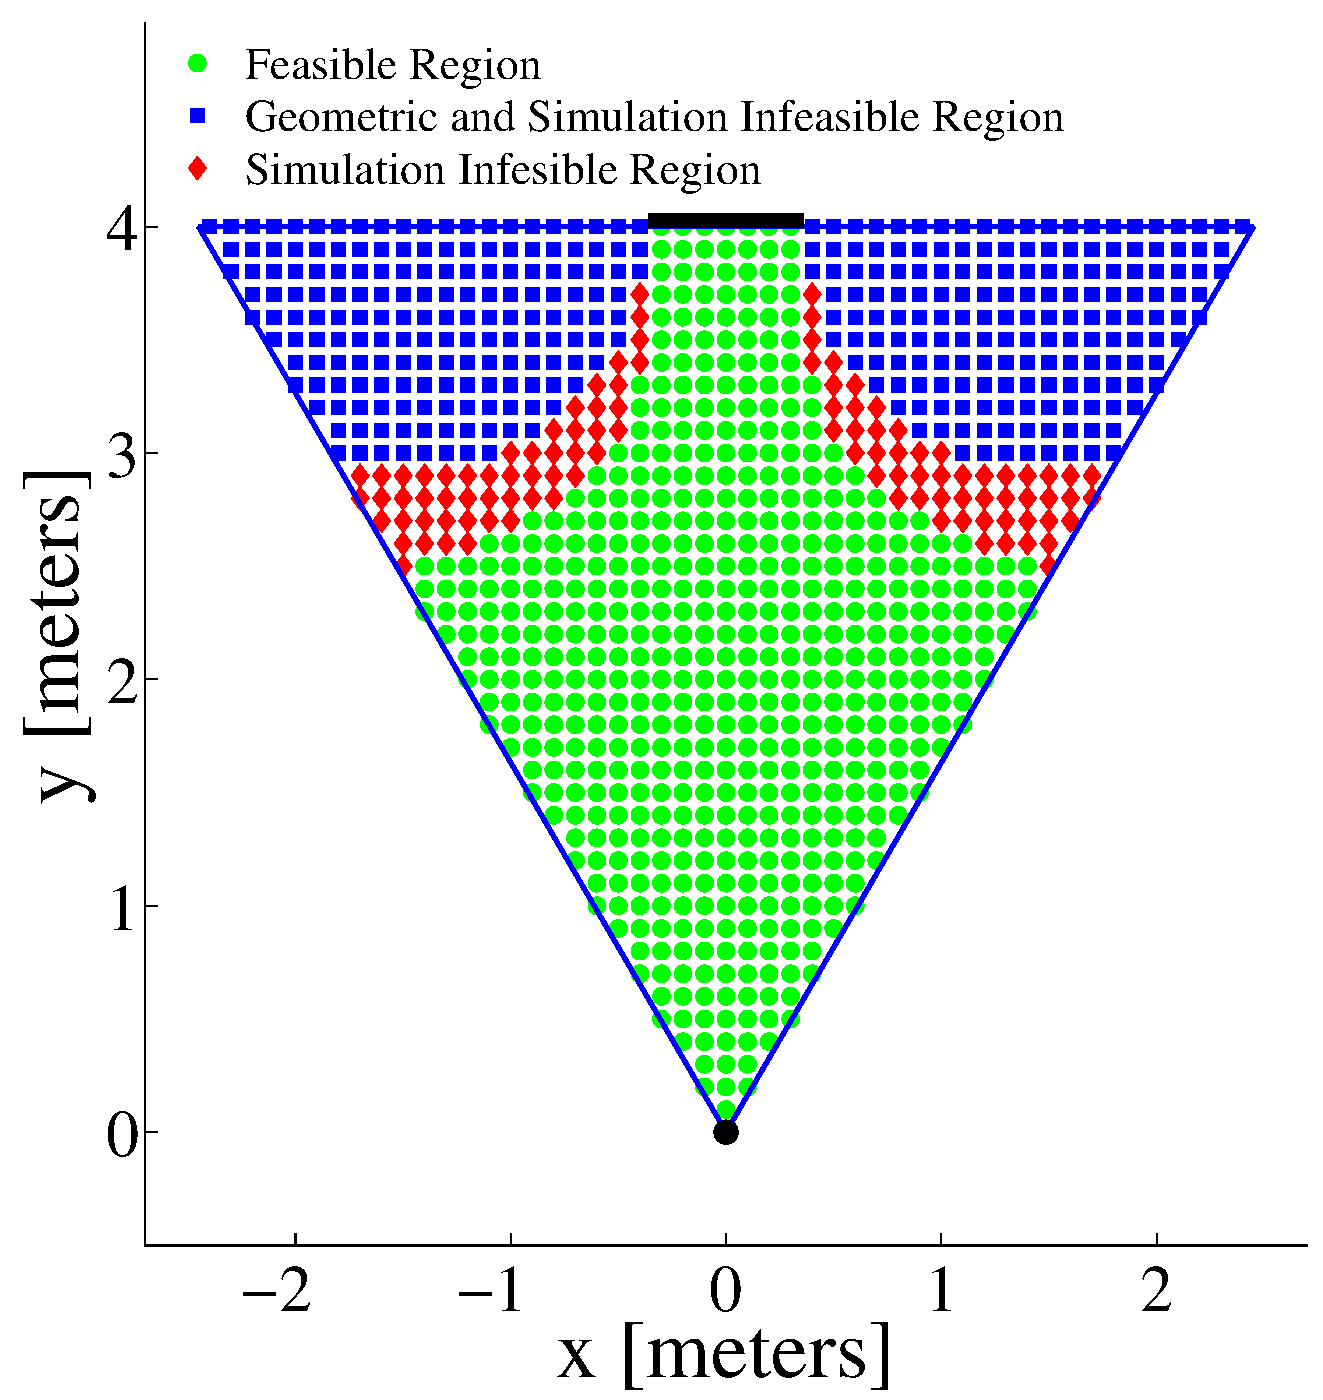
\includegraphics[width=\textwidth]{figures/feasible_set.pdf}
\caption{Plot of backwards reachable set for successful window traversal.}
\label{fig:feasible_set}
\end{minipage}
\hfill
\begin{minipage}[b]{0.45\linewidth}
\centering
\centering
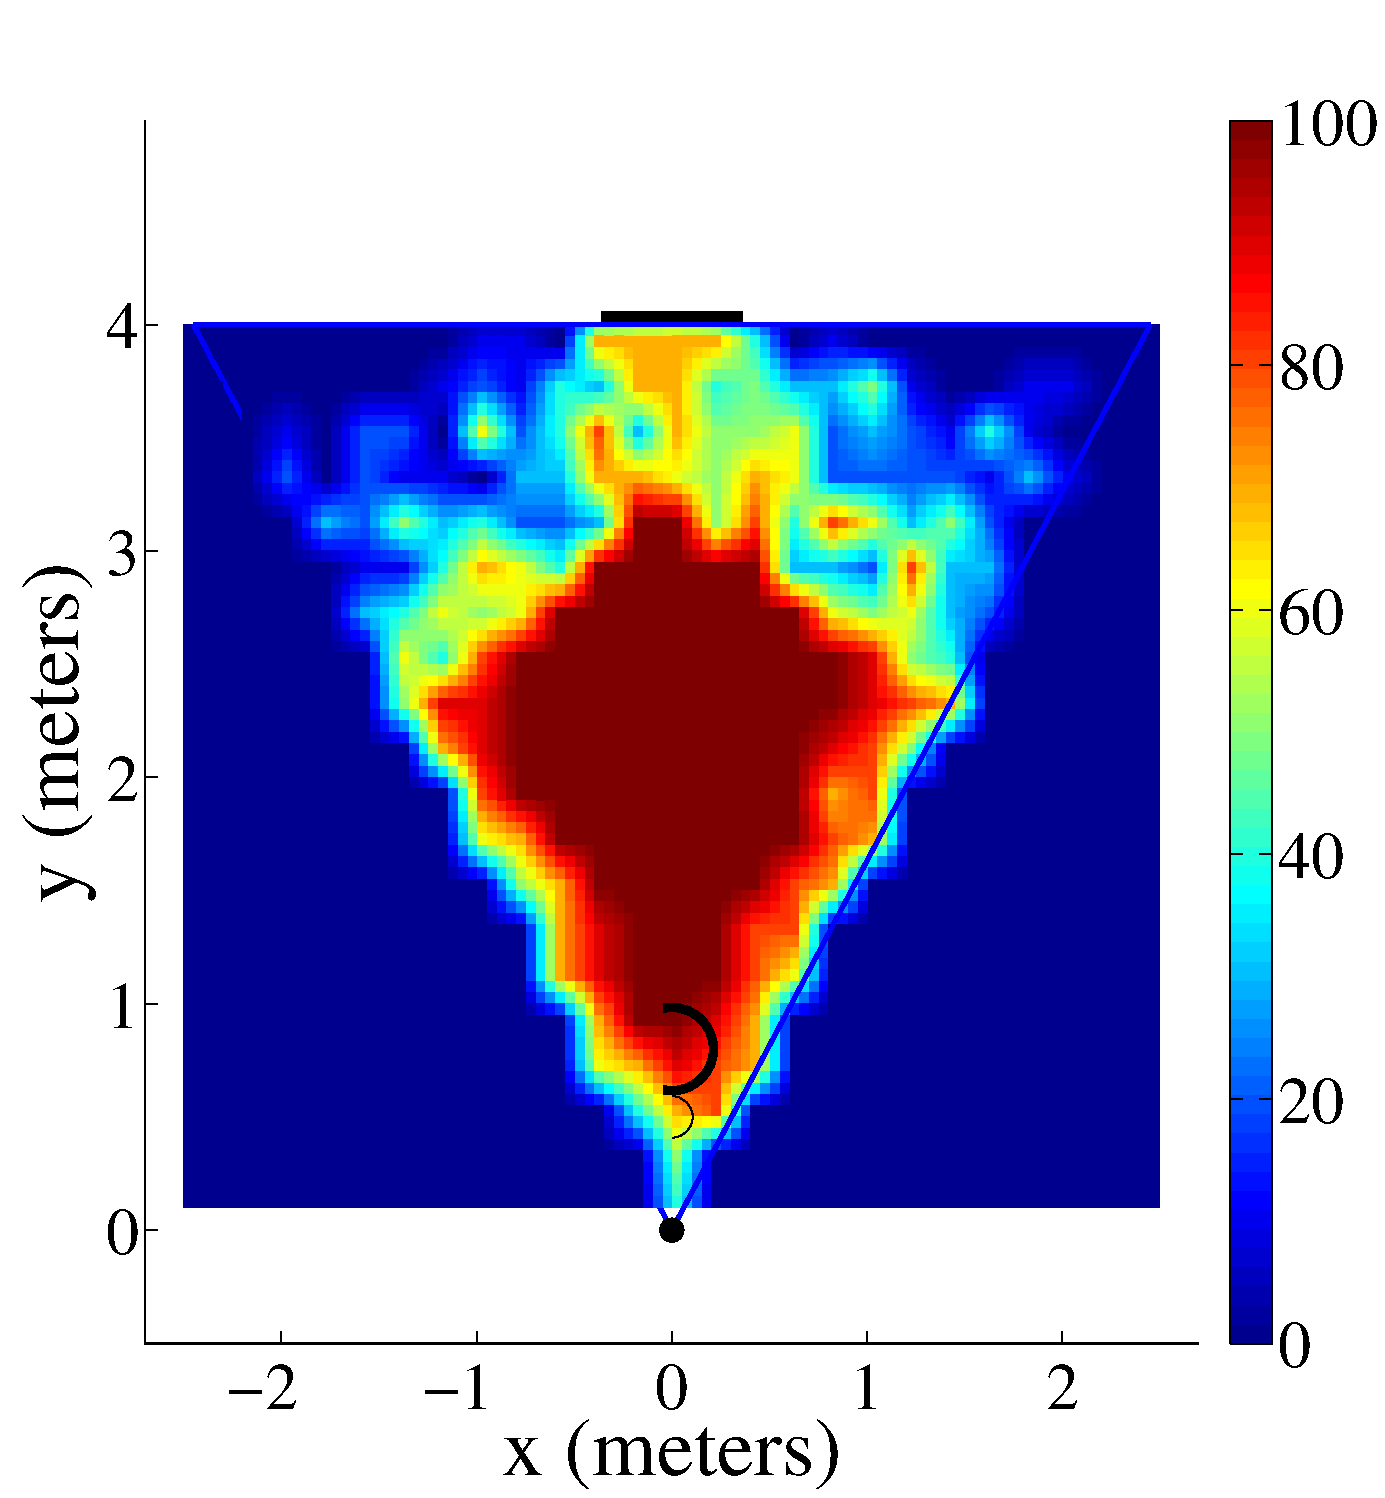
\includegraphics[width=\textwidth]{figures/heat_map.pdf}
\caption{Probability of success for all starting locations. This graphic is 
a result of a Monte Carlo simulation of the reachable set model, in which the 
initial heading of the H$^2$Bird is chosen uniformly at random from $(-90,90)$.}
\label{fig:heat_map}
\end{minipage}
\end{figure*}

We simulated the motion of the ornithopter beginning from certain positional
and angular initial conditions using several components representing the
experimental layout of our system described in Fig.~\ref{fig:block_diagram}.
For the "ornithopter dynamics" block, we used the translational model
described by~\ref{eq:total_model_plain} with the angular position model
described by~\ref{eq:transfer_func}. We tuned the PID controller for the
simulation so that paths from known positions looked similar to the behavior
we observed in the experimental data. We also inlcuded the camera capture and
pose estimation delays, and the PID controller sampling rate in the
simulation.

We determine the backwards reachable set of initial states for successful
narrow passage traversal both geometrically and in simulation
(Fig.~\ref{fig:feasible_set}). For the initial conditions, we use a uniform
grid of 0.05 meter increments within the camera viewing region, and an initial
angular position perpendicular to the narrow passage plane. The geometrically
infeasible region is computed using the minimum turning radius and the
geometry of the camera's field-of-view and is indicated in blue. Both the
regions in red and blue indicate the infeasible region determined in
simulation. The feasible region is highlighted in green. A success consisted
of a path that intersects the window at some point and does not leave the
camera viewing triangle. Fig.~\ref{fig:feasible_set} is validated by our
experimental data, as there are no successes within the geometrically
infeasible region. There are a few successes near the boundary of the
infeasible region determined in simulation, but this phenomenon can be
explained by the results in Fig.~\ref{fig:heat_map}.

Fig.~\ref{fig:heat_map} depicts the results of a Monte Carlo method of
simulating possible paths of the H$^2$Bird during our experiments. For each
point within a 0.2 meter grid within the camera viewing triangle, we simulated
10 trials using an initial heading randomly sampled from a uniform
distribution between -90$^{\circ}$ and 90$^{\circ}$. As shown in the figure,
there is a region in the middle with a 100\% probability of success, which is
a subset of the feasible region presented in Fig.~\ref{fig:feasible_set}.
Along the edges of the camera viewing triangle, however, the probability of
success decreases.

The results of our experimental trials verify the results of the Monte Carlo
simulation of the model that we used. The trials that we conducted in
Fig.~\ref{fig:flight_paths_feasible} correspond to the circled region in
Fig.~\ref{fig:heat_map}. The 80\% success rate that we experienced in the
experiments corroborates our calculated probability of success of
approximately 80\%. Additionally, the diminished success rate of 50\% near the
edges of the viewing triangle that we determined through experimentation
supports the reduced probability of success calculated by the simulation.



%%%%%%%%%%%%%%%%%%%%%%%%%%%%%%%%%%%%%%%%%%%%%%%%%%%%%%%%%%%%%%%%%%%%%%%%%%%%%%
\section{Conclusions and Future Work}
%TODO 
%%%%%%%%%%%%%%%%%%%%%%%%%%%%%%%%%%%%%%%%%%%%%%%%%%%%%%%%%%%%%%%%%%%%%%%%%%%%%%
\section{Acknowledgments}
The authors would like to thank Fernando Garcia Bermudez for his 
assistance with the Vicon motion capture system, Andrew Pullin for his 
help with robot photography, and the members of the Biomimetic 
Millisystems Laboratory and the EECS community at the University of 
California, Berkeley for their advice and support.

%%%%%%%%%%%%%%%%%%%%%%%%%%%%%%%%%%%%%%%%%%%%%%%%%%%%%%%%%%%%%%%%%%%%%%%%%%%%%%%

%%%%%%%%%%%%%%%%%%%%%%%%%%%%%%%%%%%%%%%%%%%%%%%%%%%%%%%%%%%%%%%%%%%%%%%%%%%%%%%
% BIBLIOGRAPHY

% The following two commands are all you need in the
% initial runs of your .tex file to
% produce the bibliography for the citations in your paper.
\bibliographystyle{abbrv}
\bibliography{manuscript}

% ACM needs 'a single self-contained file'!
%\subsection{References}
% Generated by bibtex from your ~.bib file.  Run latex,
% then bibtex, then latex twice (to resolve references)
% to create the ~.bbl file.  Insert that ~.bbl file into
% the .tex source file and comment out
% the command \texttt{{\char'134}thebibliography}.
\end{document}
